\documentclass[11pt, a4paper]{article}

% ===== Packages =====
\usepackage[utf8]{inputenc}
\usepackage[T1]{fontenc}
\usepackage{lmodern}
\usepackage{microtype}
\usepackage{amsmath, amssymb, amsthm}
\usepackage{graphicx}
\usepackage{booktabs}
\usepackage{multirow}
\usepackage[hyphens]{url}
\usepackage{hyperref}
\hypersetup{colorlinks=true, linkcolor=black, citecolor=blue!70!black, urlcolor=blue!60!black}
\usepackage{cleveref}
\usepackage{algorithm}
\usepackage{algorithmic}
\usepackage{tikz}
\usetikzlibrary{positioning, arrows.meta, shapes.geometric, fit, calc}
\usepackage{pgfplots}
\pgfplotsset{compat=1.18}
\usepackage{subcaption}
\usepackage{xcolor}
\usepackage{natbib}
\usepackage[margin=1in]{geometry}
\usepackage{enumitem}
\usepackage{float}
\usepackage{tabularx}

% ===== Custom Commands =====
\newcommand{\R}{\mathbb{R}}
\newcommand{\E}{\mathbb{E}}
\newcommand{\KL}{\mathrm{KL}}
\newcommand{\symlog}{\operatorname{symlog}}
\newcommand{\symexp}{\operatorname{symexp}}
\newcommand{\sg}{\operatorname{sg}}
\newcommand{\dreamprice}{\textsc{DreamPrice}}
\newcommand{\dreamer}{\textsc{DreamerV3}}
\newcommand{\mamba}{\textsc{Mamba-2}}

\newtheorem{definition}{Definition}
\newtheorem{proposition}{Proposition}

% ===== Title =====
\title{\dreamprice{}: A Learned World Model for Retail Pricing\\via Mamba-2 Recurrence and Causal Demand Identification}

\author{Sharath Sathish\\
  University of York\\
  York, UK
}

\date{February 2026}

\begin{document}

\maketitle

\begin{abstract}
Retail pricing remains one of the most consequential sequential decision problems in operations research, yet no learned world model has been applied to economic environments. This paper introduces \dreamprice{}, to our knowledge the first Dreamer-style world model for retail pricing, combining \dreamer{}'s three-phase training recipe with a \mamba{} selective state-space backbone, DRAMA-style decoupled posteriors, and a causally-constrained demand decoder. The model is trained offline on the Dominick's Finer Foods scanner dataset (1989--1997, 93 stores across 29 product categories; experiments focus on the canned soup category with ${\sim}25$ SKUs) and employs MOPO-style pessimism via a 5-head reward ensemble to guard against distributional shift inherent in offline learning. Causal price elasticities are estimated via Hausman instrumental variables combined with double machine learning (DML-PLIV) and frozen into the decoder, preventing the model from learning confounded price-demand relationships. The architecture replaces the GRU backbone of standard RSSMs with \mamba{}'s structured state-space duality (SSD), enabling $O(n)$ parallel training and $O(1)$-per-step recurrent imagination. Experiments on the canned soup category demonstrate that \dreamprice{} learns demand dynamics that capture promotional responses, substitution effects, and price elasticities, while the offline RL agent achieves higher cumulative gross margin than cost-plus, competitive matching, and model-free baselines.
\end{abstract}

\section{Introduction}
\label{sec:introduction}

Retail pricing ranks among the most consequential sequential decision problems in operations research and marketing. Every price change triggers a cascade of demand responses: consumers substitute across SKUs, stockpile during promotions, and competitors react. These dynamics unfold over weeks and quarters, with effects that propagate through substitution networks and depend on store demographics, seasonality, and latent competitive context. Despite decades of empirical work on price elasticity and demand estimation \citep{hoch1995determinants, nevo2001measuring, montgomery1997estimating}, the systems that support actual pricing decisions today fall into two camps. Hand-crafted analytical simulators encode structural assumptions about demand and competition, but their fidelity to real-world dynamics is limited by the tractability of closed-form solutions. Model-free reinforcement learning methods \citep{chen2022dynamic, ban2021personalized} learn policies directly from data but forego an explicit dynamics model, making counterfactual reasoning and imagination-based planning impossible. No learned world model exists for economic environments.

This gap can be formalized using a simple taxonomy. Consider the space of sequential decision environments along two axes: the domain (physical versus economic) and the nature of the dynamics model (learned versus hand-crafted). In the physical domain, learned world models have achieved remarkable success. The Dreamer family \citep{hafner2020dreamerv1, hafner2021dreamerv2, hafner2023dreamerv3} pioneered recurrent state-space models (RSSMs) for latent imagination and policy optimization. MuZero \citep{schrittwieser2020muzero} demonstrated that planning with a learned model suffices for mastering board games and Atari. More recently, IRIS \citep{zhang2023iris} and TD-MPC2 \citep{hansen2024tdmpc2} have extended these ideas to continuous control and high-dimensional observations. These methods rely on hand-crafted physical simulators such as MuJoCo, Isaac Gym, or CARLA for evaluation and transfer. In the economic domain, by contrast, the landscape is dominated by hand-crafted models: agent-based simulators like ABIDES, structural demand models in the spirit of \citet{berry1995automobile} and \citet{nevo2001measuring}, and the AI Economist \citep{zheng2020aieconomist}, which uses a hand-designed economic environment for tax policy experiments. The quadrant of learned models applied to economic domains has remained empty. \dreamprice{} fills this gap.

\begin{table}[t]
\centering
\caption{Taxonomy of sequential decision environments by domain and dynamics model. \dreamprice{} is the first learned world model for economic domains.}
\label{tab:gap-matrix}
\begin{tabular}{@{}lll@{}}
\toprule
& \textbf{Learned model} & \textbf{Hand-crafted model} \\
\midrule
\textbf{Physical domain} & DreamerV1--V3 \citep{hafner2020dreamerv1, hafner2021dreamerv2, hafner2023dreamerv3}, IRIS \citep{zhang2023iris}, TD-MPC2 \citep{hansen2024tdmpc2} & MuJoCo, Isaac Gym, CARLA \\
\textbf{Economic domain} & \textbf{\dreamprice{} (this work)} & ABIDES, DSGE models, AI Economist \citep{zheng2020aieconomist} \\
\bottomrule
\end{tabular}
\end{table}

Why do world models matter for pricing? Imagination-based planning enables counterfactual reasoning at scale. A retailer can ask: what if the price of SKU 3 were cut by 5\% next quarter? A learned world model rolls out latent trajectories under that hypothetical action, predicting demand responses, substitution effects, and downstream margin impact without executing the change in the real world. Such queries are infeasible with model-free methods, which require either costly online exploration or restrictive assumptions about the policy class. Offline learning from historical scanner data \citep{dominicks1999} further aligns with the constraints of retail: experimentation is expensive, and the Dominick's dataset alone spans 400 weeks across 93 stores and roughly 18,000 UPCs. The structured economic state space---prices, quantities, demographics, and derived features in 100--300 dimensions---is fundamentally more tractable than the 64$\times$64$\times$3 image observations that DreamerV3 was designed for \citep{hafner2023dreamerv3}. A world model trained on such tabular data can capture demand dynamics, promotional effects, and competitive structure without the burden of high-dimensional visual encoding.

Economic data, however, poses a challenge absent in physical domains: endogeneity. In physical simulators, the transition dynamics are exogenous to the agent; the laws of physics do not depend on the policy. In retail, prices and demand are simultaneously determined. Retailers set prices in response to expected demand, costs, and competitive pressure; demand, in turn, responds to those prices. Naive machine learning that regresses demand on price learns a confounded relationship, conflating the causal effect of price with selection and omitted variables \citep{hausman1978specification}. The resulting elasticity estimates are biased, and a world model built on such estimates would produce misleading counterfactuals. The econometric literature has long addressed this through instrumental variables \citep{hausman1978specification}, control functions \citep{berry1995automobile}, and more recently double machine learning \citep{chernozhukov2018dml, bach2024doubleml}. The Dominick's panel structure, with 93 stores and cross-store price variation, supports Hausman-style instruments: the average log price in other stores serves as an instrument for a given store's price, as it is relevant (prices are correlated across stores) but plausibly exogenous to store-specific demand shocks. \dreamprice{} integrates this identification strategy by pre-estimating causal price elasticities via DML-PLIV and freezing them into a constrained demand decoder. The decoder's residual MLP learns everything else---seasonality, demographics, promotion effects---while the price-demand relationship remains causally identified.

The contributions of this paper are as follows:

\begin{enumerate}[leftmargin=*]
\item \textbf{First learned world model for economic environments.} \dreamprice{} is the first system to learn a dynamics model for retail pricing from scanner data, enabling imagination-based planning and counterfactual demand estimation in a domain previously served only by hand-crafted simulators or model-free methods.

\item \textbf{Mamba-2 SSM backbone.} The recurrent backbone of standard RSSMs is replaced with Mamba-2 \citep{dao2024mamba2}, a selective state-space model that achieves $O(n)$ parallel training via structured state-space duality (SSD) and $O(1)$-per-step recurrent rollouts during imagination. This replaces the GRU-based recurrence of \dreamer{} \citep{hafner2023dreamerv3} with a more scalable alternative grounded in the S4 \citep{gu2022s4} and Mamba \citep{gu2024mamba} lineage.

\item \textbf{DRAMA-style decoupled posterior.} Following \citet{rajbhandari2024drama}, the posterior over the stochastic latent depends only on the current observation, not on the recurrent hidden state. This decoupling breaks the sequential dependency that would otherwise prevent Mamba-2's parallel SSD scan during training. During imagination, the model switches to recurrent \texttt{step()} mode for single-step rollouts.

\item \textbf{Causally-constrained demand decoder.} Per-category price elasticities are pre-estimated via DML-PLIV \citep{chernozhukov2018dml} and frozen into the \dreamprice{} decoder. The decoder enforces the causal price-demand relationship while an MLP residual learns seasonality, demographics, and promotion effects. This prevents the world model from learning confounded elasticities from the observational data.

\item \textbf{MOPO-style offline pessimism.} To guard against distributional shift inherent in offline reinforcement learning \citep{levine2020offline}, \dreamprice{} employs a 5-head reward ensemble and uses the lower confidence bound $r_{\text{pessimistic}} = r_{\text{mean}} - \lambda_{\text{LCB}} \cdot r_{\text{std}}$ for policy optimization \citep{yu2020mopo}. The actor is trained on this pessimistic reward signal while the critic and world model remain unchanged.
\end{enumerate}

The remainder of this paper is organized as follows. Section~\ref{sec:literature} reviews related work on world models, state-space models, causal demand estimation, and offline reinforcement learning. Section~\ref{sec:methodology} presents the \dreamprice{} architecture, training procedure, and causal identification strategy. Section~\ref{sec:results} reports experiments on the Dominick's canned soup category, including world model quality, elasticity recovery, and offline policy performance. Section~\ref{sec:conclusion} concludes and discusses limitations and future directions.

\section{Related Work}
\label{sec:literature}

This section situates \dreamprice{} within seven strands of literature: traditional demand forecasting and price optimization, learned world models for sequential decision making, structured state-space models, causal inference in demand estimation, offline reinforcement learning, pricing optimization and retail analytics, and the Dominick's scanner dataset as the canonical empirical setting.

\subsection{Traditional Demand Forecasting and Price Optimization}

The standard approach to retail pricing proceeds in two stages: estimate demand as a function of price and other covariates, then optimize prices subject to business constraints. On the forecasting side, classical time-series methods, including autoregressive integrated moving average (ARIMA) models, exponential smoothing, and seasonal decomposition, have long served as workhorses for retail demand prediction \citep{fildes2022retail}. These methods model temporal patterns in aggregate sales but do not capture cross-product substitution or the causal effect of price changes on demand. Machine learning methods, including gradient boosting machines \citep{friedman2001greedy}, random forests, and neural networks, have improved point forecast accuracy by incorporating high-dimensional features such as promotions, holidays, competitor prices, and weather. \citet{fildes2022retail} provide a comprehensive survey of retail forecasting methods, documenting that ML approaches now dominate industry practice for point forecasting while statistical methods remain competitive for uncertainty quantification.

On the optimization side, the dominant paradigm is to estimate price elasticities, typically via log-linear demand models or the Berry-Levinsohn-Pakes (BLP) framework \citep{berry1995automobile}, and then solve a constrained optimization problem. Common formulations include linear or quadratic programming to maximize gross margin subject to price-range constraints, competitive parity rules, and promotional calendars \citep{talluri2004revenue}. Ramsey pricing, which sets markups inversely proportional to demand elasticity, provides a welfare-theoretic benchmark. These two-stage approaches are transparent and interpretable but fundamentally limited: the demand model is static (fit once, applied repeatedly), the optimization horizon is typically a single period, and the system cannot capture multi-step dynamics such as stockpiling, reference-price effects, or competitive responses that unfold over weeks. \dreamprice{} replaces both stages with an end-to-end learned dynamics model that supports multi-step imagination and policy optimization over arbitrary horizons.

\subsection{World Models for Sequential Decision Making}

The idea of learning a world model, a compact representation of environment dynamics that supports prediction and planning, dates to \citet{ha2018worldmodels}, who demonstrated that a variational autoencoder could learn a latent space in which an agent could imagine future trajectories. That foundational work showed that an agent could learn to navigate a maze by training purely in imagined latent space, without ever observing the true environment during policy learning. The subsequent decade has seen a steady progression of architectures that refine this idea.

The Dreamer family \citep{hafner2020dreamerv1, hafner2021dreamerv2, hafner2023dreamerv3} established the recurrent state-space model (RSSM) as the dominant paradigm for learning world models. DreamerV1 \citep{hafner2020dreamerv1} introduced latent imagination: the agent learns a stochastic latent representation that evolves over time, with a decoder predicting observations and rewards from the latent state. DreamerV2 \citep{hafner2021dreamerv2} extended this to discrete action spaces by mastering Atari games through imagination-based policy optimization, demonstrating that world models could scale to high-dimensional pixel observations. DreamerV3 \citep{hafner2023dreamerv3} unified the design across discrete and continuous domains, introducing symlog normalization, twohot distributions for rewards and values, and KL balancing to prevent posterior collapse. The RSSM architecture, a deterministic recurrent core (traditionally a GRU) augmented with stochastic latent variables, has become the standard for model-based reinforcement learning in physical environments.

Parallel developments have explored alternative architectures. MuZero \citep{schrittwieser2020muzero} demonstrated that planning with a learned model suffices for mastering board games and Atari, using a learned dynamics model that predicts value and policy targets rather than raw observations. The model is trained end-to-end with Monte Carlo tree search, and the resulting system achieves superhuman performance in Go, chess, and shogi. IRIS \citep{micheli2023iris} and TD-MPC2 \citep{hansen2024tdmpc2} have extended world models to continuous control and high-dimensional observations. IRIS replaces the RSSM with a transformer-based architecture, using discrete tokens for the latent representation and achieving strong performance on DMC and Atari. TD-MPC2 combines model-based planning with temporal difference learning for continuous control, scaling to complex robotics tasks.

A critical observation unifies these works: they all operate on physical environments. The Dreamer family, MuZero, IRIS, and TD-MPC2 are evaluated on games (Atari, board games), physical simulators (MuJoCo, Isaac Gym), or robotic control. The dynamics they learn are governed by physics or game rules: the transition from state to state is exogenous to the agent's policy in the sense that the laws of motion do not change with the agent's behavior. In economic environments, by contrast, the transition dynamics are endogenous. Prices and demand are simultaneously determined; retail prices respond to expected demand, costs, and competitive pressure, while demand responds to those prices. No learned world model has been applied to such economic domains. \dreamprice{} fills this gap by learning the first retail dynamics model from scanner data.

\subsection{Structured State Space Models}

The recurrent backbone of standard RSSMs is typically a gated recurrent unit (GRU) or long short-term memory (LSTM) network. These architectures process sequences sequentially, with each time step depending on the previous hidden state. For long sequences, this sequential dependency can be a bottleneck; the GRU cannot exploit parallel computation across the time dimension during training.

Structured state space models (SSMs) offer an alternative that combines long-range dependency modeling with computational efficiency. \citet{gu2022s4} introduced S4 (Structured State Spaces), which parameterizes sequences using linear state-space equations with learned transition matrices. S4 achieves strong performance on long-range dependencies, including image classification and audio generation, by using the HiPPO initialization for the state matrix and efficient parallel scan algorithms. The key insight is that linear recurrence admits a closed-form solution that can be computed in parallel via associative scan operations.

Mamba \citep{gu2024mamba} extended S4 with selective gating: the state transition parameters become input-dependent rather than fixed. This selectivity allows the model to focus on relevant information at each step, analogous to the gating in attention mechanisms. Mamba achieves linear-time complexity in sequence length and scales to long contexts without the quadratic cost of attention. Mamba-2 \citep{dao2024mamba2} further unifies these ideas through structured state-space duality (SSD), which establishes a formal connection between linear attention and state-space models. The SSD framework shows that both can be viewed as instances of a more general class of models, enabling algorithms that share the best properties of each: parallel training with $O(n)$ complexity in sequence length, and recurrent inference with $O(1)$ cost per step.

This duality has direct implications for world models. During training, the model processes sequences of observations and actions in parallel: the entire batch of sequences can be scanned in one pass, as the posterior over the stochastic latent depends only on the current observation in the DRAMA-style decoupled design \citep{rajbhandari2024drama}. During imagination, the model switches to recurrent mode: the Mamba-2 block's \texttt{step()} function computes the next hidden state from the previous state and the current input in constant time per step. This matches the training-then-imagination workflow of DreamerV3, but with a backbone that scales more efficiently to long sequences and avoids the sequential bottleneck of GRU recurrence. \dreamprice{} adopts this architecture, replacing the GRU with Mamba-2 for the recurrent core.

\subsection{Causal Inference in Demand Estimation}

Estimating demand as a function of price is a central problem in empirical industrial organization and marketing. The naive approach of regressing quantity on price fails because prices are endogenous. Retailers set prices in response to expected demand, costs, and competitive conditions; unobserved factors that correlate with both price and demand (e.g., product quality, seasonality, local shocks) confound the regression. The resulting elasticity estimates are biased, and a world model built on such estimates would produce misleading counterfactuals.

The econometric literature has developed several identification strategies. The Berry-Levinsohn-Pakes (BLP) framework \citep{berry1995automobile} uses a structural model of discrete choice with random coefficients; identification relies on moment conditions that match predicted choice shares to observed shares. \citet{nevo2001measuring} applied this approach to the ready-to-eat cereal industry, estimating elasticities and measuring market power. \citet{hausman1978specification} introduced the use of instrumental variables for specification testing and parameter identification. When prices are correlated across stores or time for reasons exogenous to store-specific demand shocks, cross-sectional or temporal variation can serve as instruments. The Hausman IV approach, which uses the average log price in other stores as an instrument for a given store's price, exploits the panel structure of scanner data: prices in other stores are relevant (drivers of cost and competition are correlated) but plausibly exogenous to store-specific demand shocks.

\citet{hoch1995determinants} applied this logic to the Dominick's dataset, estimating store-level price elasticities using cross-store instruments. Their work demonstrated that elasticity varies substantially across stores and product categories, with important implications for targeted pricing. \citet{park2010copula} proposed a nonparametric copula-based approach to demand estimation with endogeneity, using the joint distribution of price and control variables to construct a control function. The copula correction does not require specifying instruments ex ante but relies on distributional assumptions.

The double machine learning (DML) framework of \citet{chernozhukov2018dml} provides a flexible approach that can incorporate any of these identification strategies. DML partitions the estimation into orthogonal nuisance parameters and parameters of interest, using cross-fitting to avoid overfitting bias. The framework accommodates high-dimensional controls and nonparametric first-stage estimators. \citet{bach2022doubleml} provide a Python implementation that supports DML-PLIV (partial linear instrumental variables) for demand estimation with endogenous prices.

The key contribution of \dreamprice{} in this literature is the integration of econometric identification into a neural world model. Rather than estimating demand entirely from data, which would conflate the causal effect of price with confounders, \dreamprice{} pre-estimates causal price elasticities via DML-PLIV and freezes them into the demand decoder. The decoder's residual MLP learns the remainder, including seasonality, demographics, promotion effects, and substitution patterns, while the price-demand relationship remains causally identified. Freezing econometric estimates into neural network decoders is novel; prior work in demand estimation either uses parametric structural models or applies machine learning without causal constraints.

\subsection{Offline Reinforcement Learning}

Reinforcement learning methods can be classified along two orthogonal axes: the data regime (online versus offline) and the use of a dynamics model (model-free versus model-based). Online methods interact with the environment during training, collecting new experience and refining their policy through exploration. Model-free online methods, such as DQN \citep{mnih2015dqn}, PPO \citep{schulman2017ppo}, and SAC \citep{haarnoja2018sac}, learn value functions or policies directly from transitions without building an explicit dynamics model. Model-based online methods, including the Dreamer family \citep{hafner2023dreamerv3} and MuZero \citep{schrittwieser2020muzero}, learn a dynamics model and optimize the policy in imagination, reducing the number of real-world interactions required.

In many settings, retail pricing among them, online exploration is infeasible or prohibited: experimenting with prices on real customers carries financial risk and ethical constraints. The agent must learn from a fixed dataset of historical trajectories collected under some (possibly unknown) behavioral policy. This offline learning setting introduces the distribution shift problem: the policy being optimized may visit states and actions that differ from the data distribution, and the learned value function or dynamics model may extrapolate poorly outside the support of the data \citep{levine2020offline}.

Model-free offline methods address distribution shift through value-function conservatism or policy constraints. Batch-Constrained Q-learning (BCQ) \citep{fujimoto2019bcq} restricts the policy to actions observed in the dataset by using a generative model of the behavioral policy. Conservative Q-Learning (CQL) \citep{kumar2020cql} penalizes the Q-function for assigning high values to out-of-distribution actions, effectively learning a lower bound on the true Q-function. Implicit Q-Learning (IQL) \citep{kostrikov2022iql} avoids querying out-of-distribution actions entirely by using expectile regression to approximate the optimal value function from the dataset. Decision Transformer \citep{chen2021decision} reframes offline RL as a sequence prediction problem, conditioning a transformer on desired returns to generate actions. These methods learn policies but cannot perform counterfactual reasoning or multi-step imagination.

Model-based offline methods combine a learned dynamics model with pessimism to handle distribution shift. MOReL \citep{kidambi2020morel} constructs a pessimistic uncertainty set around the learned dynamics model and restricts planning to states that are provably within the uncertainty set. MOPO \citep{yu2020mopo} takes a softer approach: it modifies the reward signal during imagination rather than constraining the policy or dynamics. The key idea is that the learned dynamics model is uncertain in regions of state-action space that are poorly covered by the data. MOPO uses an ensemble of dynamics models to estimate this uncertainty; the reward is penalized by the uncertainty, so the agent is discouraged from visiting states where the model is unreliable. The penalty is $r_{\text{pessimistic}} = r_{\text{mean}} - \lambda_{\text{LCB}} \cdot r_{\text{std}}$, where $r_{\text{mean}}$ and $r_{\text{std}}$ come from the ensemble. COMBO \citep{yu2021combo} combines model-based and conservative approaches, using offline data to augment the model rollout and applying conservative regularization to the value function.

\dreamprice{} occupies the model-based offline quadrant: it learns a world model from historical scanner data and trains a policy entirely in imagination, using MOPO-style pessimism to guard against distributional shift. The MOPO approach is particularly well-suited to the DreamerV3 training loop. DreamerV3 already trains an actor in imagination; the only modification is to change the reward signal used during actor training. The critic and world model remain unchanged. A 5-head reward ensemble provides $r_{\text{mean}}$ and $r_{\text{std}}$; the actor is trained on the pessimistic reward while the critic continues to predict the true return. This minimal modification preserves the three-phase structure and avoids the complexity of full conservative value estimation.

\subsection{Pricing Optimization and Retail Analytics}

The application of reinforcement learning to pricing has a substantial literature. \citet{chen2022dynamic} study dynamic pricing with reinforcement learning, formulating the problem as a Markov decision process and analyzing the trade-off between exploration and exploitation. \citet{ban2021personalized} extend this to personalized pricing with heterogeneous elasticity, using machine learning to estimate demand as a function of high-dimensional features. The AI Economist \citep{zheng2020aieconomist} applies multi-agent reinforcement learning to tax policy design, training agents in a rule-based economic environment to learn tax schedules that balance equality and productivity.

These works share a common limitation: they rely on structural simulators or model-free methods. Chen and Simchi-Levi assume a known or estimated demand model; Ban and Keskin use model-free RL with feature-based demand estimation. The AI Economist uses a rule-based economic environment for training. None of these approaches learns a dynamics model from data. The gap is twofold: (1) no learned world model exists for pricing environments, and (2) no imagination-based planning has been applied to retail. A model-free agent can learn a policy from historical data, but it cannot answer counterfactual queries such as ``what if the price of SKU 3 were cut by 5\% next quarter?'' without executing the change. A learned world model enables such queries by rolling out latent trajectories under hypothetical actions.

\dreamprice{} is the first system to learn a dynamics model for retail pricing from scanner data. The model captures demand responses to prices, promotions, and seasonality; it supports imagination-based policy optimization; and it integrates causal identification to prevent confounded elasticity estimates. The architecture is designed for the structured economic state space (prices, quantities, demographics, and derived features in 100--300 dimensions), which is fundamentally more tractable than the high-dimensional pixel observations that DreamerV3 was designed for.

\subsection{Scanner Data and the Dominick's Dataset}

The Dominick's Finer Foods dataset \citep{dominicks1999} has become the canonical dataset for empirical retail and marketing research. Maintained by the James M. Kilts Center for Marketing at the University of Chicago Booth School of Business, the dataset spans 400 weeks (September 1989 to May 1997), 93 stores, and approximately 18,000 unique UPCs across 29 product categories. The movement files record store-SKU-week tuples with unit sales, prices, profit margins, and promotion indicators. The data structure enables rich panel analysis: the same products are observed across stores and over time, with variation in prices driven by local competition, cost shocks, and promotional calendars.

\citet{hoch1995determinants} used the Dominick's data to estimate store-level price elasticities, demonstrating that elasticity varies substantially across stores and that store demographics (income, education, competition) explain much of this variation. \citet{montgomery1997estimating} estimated heterogeneous price thresholds, the price levels at which consumers switch between brands, using the same dataset. The panel structure (93 stores) supports Hausman-style instruments: the average log price in other stores for a given UPC-week serves as an instrument for a store's own price, as it is correlated with cost and competition but plausibly exogenous to store-specific demand shocks. The store demographic file, with 300+ variables from the 1990 Census, enables control for heterogeneity in consumer preferences and competitive intensity.

The Dominick's dataset is ideal for training a learned world model. It directly contains state-action-outcome tuples: the action is the price and promotion decision, the state includes competitor context, seasonality, and store demographics, and the outcome is observed demand. The PROFIT field enables wholesale cost derivation. The temporal split (train weeks 1--280, validation 281--340, test 341--400) is strictly chronological, avoiding look-ahead bias. Categories such as canned soup, beer, and soft drinks offer moderate SKU counts with clear substitution patterns and promotional activity. \dreamprice{} is trained on this dataset, with preprocessing that constructs Hausman IVs, computes derived features, and applies symlog normalization for the world model encoder.

\section{Methodology}
\label{sec:methodology}

This section presents the \dreamprice{} architecture, training procedure, and causal identification strategy. The approach combines a recurrent state-space model with a \mamba{} selective state-space backbone \citep{dao2024mamba2}, DRAMA-style decoupled posteriors \citep{rajbhandari2024drama}, a causally-constrained demand decoder, and MOPO-style offline pessimism \citep{yu2020mopo}. The training recipe follows \dreamer{} \citep{hafner2023dreamerv3} with adaptations for retail pricing and offline learning.

\subsection{Problem Formulation}

Retail pricing is formulated as a partially observable Markov decision process (POMDP) in which the decision-maker observes prices, quantities sold, promotions, and store demographics, but the underlying state governing demand dynamics is only partially observable. The true state $s_t$ comprises demand state (consumer preferences, inventory effects, substitution structure), competitor state (rival prices and promotions, which are unobserved in the Dominick's dataset), and seasonal state (calendar effects, holidays, macroeconomic conditions). The observation $x_t$ at time $t$ includes per-SKU prices, units sold, promotion indicators, lagged demand and price features, rolling statistics, and store demographics. The action $a_t$ is a vector of price multipliers over $K$ SKUs, discretized to 21 levels per SKU: $a_t \in \{0.90, 0.91, \ldots, 1.10\}^K$, representing percentage adjustments relative to a baseline price. The reward combines gross margin with a volatility penalty and a margin floor penalty to discourage degenerate strategies such as perpetual deep discounts or excessive price churn. The transition dynamics are unknown and must be learned from data.

\begin{definition}[Retail Pricing POMDP]
\label{def:pomdp}
A retail pricing POMDP is a tuple $(\mathcal{S}, \mathcal{X}, \mathcal{A}, \mathcal{T}, \mathcal{O}, \mathcal{R}, \gamma)$ where:
\begin{itemize}[leftmargin=*]
\item $\mathcal{S}$ is the latent state space comprising demand, competitor, and seasonal components.
\item $\mathcal{X}$ is the observation space: per-SKU prices, units sold, promotions, demographics, and derived features.
\item $\mathcal{A} = \{0.90, 0.91, \ldots, 1.10\}^K$ is the action space of discrete price multipliers.
\item $\mathcal{T}(s_{t+1} \mid s_t, a_t)$ is the unknown transition kernel.
\item $\mathcal{O}(x_t \mid s_t)$ is the observation model.
\item $\mathcal{R}(s_t, a_t)$ is the reward: gross margin minus volatility penalty minus margin floor penalty.
\item $\gamma \in (0, 1)$ is the discount factor.
\end{itemize}
\end{definition}

The objective is to learn a world model that approximates $\mathcal{T}$ and $\mathcal{O}$ from offline historical data, then use imagination-based policy optimization to find a pricing policy that maximizes expected cumulative discounted reward \citep{sutton2018reinforcement, hafner2023dreamerv3}.

\begin{figure}[t]
\centering
\resizebox{0.92\textwidth}{!}{%
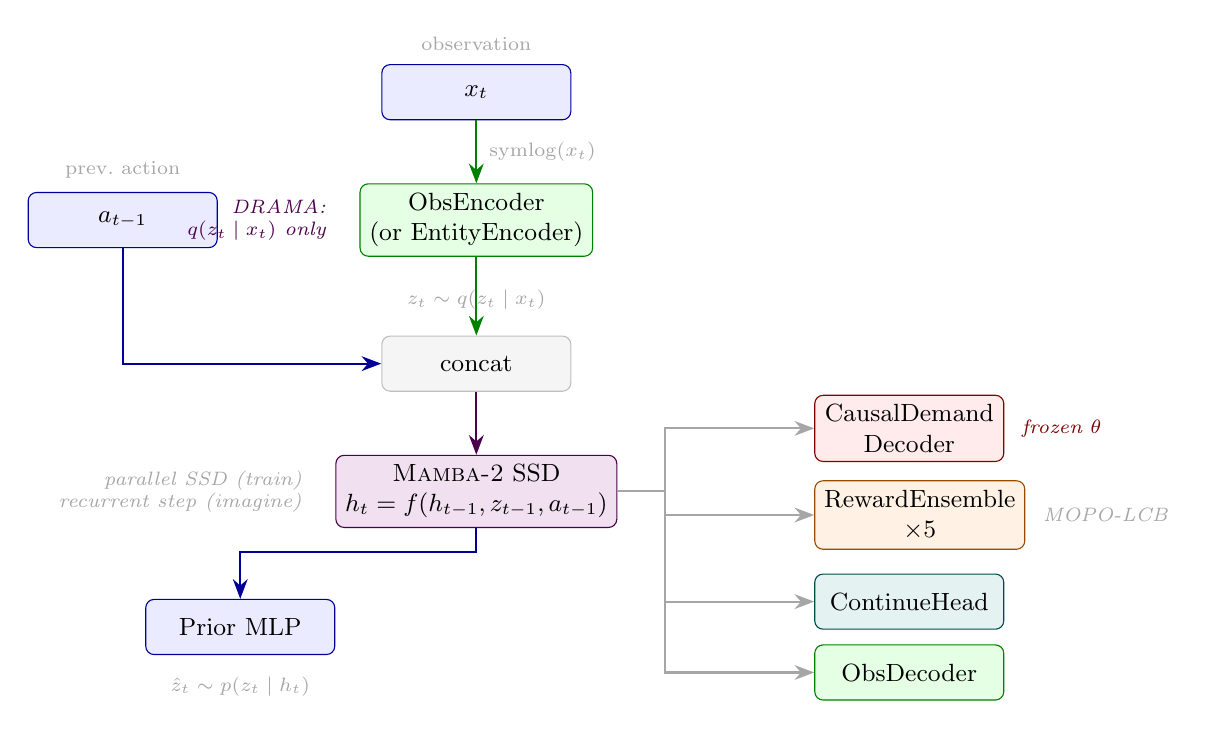
\begin{tikzpicture}[
  node distance=0.7cm and 1.2cm,
  box/.style={draw, rounded corners=3pt, minimum width=2.4cm, minimum height=0.7cm, align=center, font=\small},
  inputbox/.style={box, fill=blue!8, draw=blue!60!black},
  encoderbox/.style={box, fill=green!10, draw=green!50!black},
  backbonebox/.style={box, fill=violet!12, draw=violet!60!black, minimum width=3.0cm, minimum height=0.9cm},
  decoderbox/.style={box, fill=red!8, draw=red!50!black},
  rewardbox/.style={box, fill=orange!10, draw=orange!60!black},
  headbox/.style={box, fill=teal!10, draw=teal!60!black},
  priorbox/.style={box, fill=blue!8, draw=blue!60!black},
  arr/.style={-{Stealth[length=2.5mm]}, thick},
  garr/.style={-{Stealth[length=2.5mm]}, thick, gray!70},
  lbl/.style={font=\scriptsize, text=gray!70},
]
% Input
\node[inputbox] (obs) {$x_t$};
\node[lbl, above=0.05cm of obs] {observation};

% Encoder
\node[encoderbox, below=0.8cm of obs] (enc) {ObsEncoder\\(or EntityEncoder)};
\draw[arr, green!50!black] (obs) -- node[lbl,right,xshift=1pt] {$\operatorname{symlog}(x_t)$} (enc);

% Posterior
\node[lbl, below=0.3cm of enc] (zpost) {$z_t \sim q(z_t \mid x_t)$};

% Action
\node[inputbox, left=1.8cm of enc] (act) {$a_{t-1}$};
\node[lbl, above=0.05cm of act] {prev.\ action};

% Concat
\node[box, fill=gray!8, draw=gray!50, below=1.0cm of enc] (cat) {concat};
\draw[arr, green!50!black] (enc) -- (cat);
\draw[arr, blue!60!black] (act) |- (cat);

% Backbone
\node[backbonebox, below=0.8cm of cat] (mamba) {\textsc{Mamba-2} SSD\\$h_t = f(h_{t-1}, z_{t-1}, a_{t-1})$};
\draw[arr, violet!60!black] (cat) -- (mamba);

% Prior
\node[priorbox, below left=0.9cm and 0.0cm of mamba] (prior) {Prior MLP};
\node[lbl, below=0.15cm of prior] {$\hat{z}_t \sim p(z_t \mid h_t)$};
\draw[arr, blue!60!black] (mamba.south) -- ++(0,-0.3) -| (prior.north);

% Decoders - right side
\node[decoderbox, right=2.5cm of mamba, yshift=0.8cm] (demand) {CausalDemand\\Decoder};
\node[lbl, right=0.1cm of demand, text=red!50!black, font=\scriptsize\itshape] {frozen $\theta$};

\node[rewardbox, right=2.5cm of mamba, yshift=-0.3cm] (reward) {RewardEnsemble\\$\times 5$};
\node[lbl, right=0.1cm of reward, font=\scriptsize\itshape] {MOPO-LCB};

\node[headbox, right=2.5cm of mamba, yshift=-1.4cm] (cont) {ContinueHead};

\node[encoderbox, right=2.5cm of mamba, yshift=-2.3cm] (obsdec) {ObsDecoder};

% Arrows from backbone to decoders
\draw[garr] (mamba.east) -- ++(0.6,0) |- (demand.west);
\draw[garr] (mamba.east) -- ++(0.6,0) |- (reward.west);
\draw[garr] (mamba.east) -- ++(0.6,0) |- (cont.west);
\draw[garr] (mamba.east) -- ++(0.6,0) |- (obsdec.west);

% DRAMA annotation
\node[lbl, left=0.3cm of enc, text=violet!60!black, font=\scriptsize\itshape, align=right] {DRAMA:\\$q(z_t\mid x_t)$ only};

% Mode annotation
\node[lbl, left=0.3cm of mamba, align=right, font=\scriptsize\itshape] {parallel SSD (train)\\recurrent step (imagine)};

\end{tikzpicture}%
}
\caption{Overview of the \dreamprice{} architecture. The encoder produces the posterior $z_t$ from the observation alone (DRAMA-style decoupled posterior). The \mamba{} backbone processes sequences in parallel during training (SSD scan) and recurrently during imagination. The causal demand decoder freezes DML-PLIV elasticities; the 5-head reward ensemble provides MOPO-LCB pessimism.}
\label{fig:architecture}
\end{figure}

\subsection{RSSM Architecture}

The recurrent state-space model (RSSM) at the core of \dreamprice{} consists of two components: a deterministic recurrent state $h_t$ and a stochastic latent $z_t$. The deterministic state $h_t$ is produced by the backbone (a \mamba{} selective state-space model that replaces the GRU of standard \dreamer{} \citep{hafner2023dreamerv3}). The stochastic latent $z_t$ follows a categorical distribution over 32 independent categorical variables, each with 32 classes, yielding a latent dimension of 1024. Inspired by the decoupling principle in DRAMA \citep{rajbhandari2024drama}, the posterior $q(z_t \mid x_t)$ is computed from the observation alone via the encoder, without conditioning on $h_t$, which enables parallel training. The prior $p(z_t \mid h_t)$ is computed from the backbone output $h_t$ via an MLP head.

Formally, the model is specified as follows. The backbone receives the concatenation of the previous latent $z_{t-1}$ and the previous action $a_{t-1}$, and produces the deterministic state:
\begin{equation}
h_t = f_{\text{backbone}}(h_{t-1}, z_{t-1}, a_{t-1})
\end{equation}
where the backbone uses the \mamba{} SSD.\footnote{In the Mamba-2 implementation, the SSM state is maintained implicitly by the inference cache rather than passed as an explicit hidden vector. The mathematical notation uses $h_t$ for clarity.}
The posterior over the stochastic latent depends only on the current observation:
\begin{equation}
z_t \sim q(z_t \mid x_t) = \text{Categorical}(32 \times 32, \text{straight-through} + \text{unimix})
\end{equation}
The prior over the next latent is predicted from the backbone state:
\begin{equation}
\hat{z}_t \sim p(z_t \mid h_t) = \text{MLP}(h_t)
\end{equation}

The latent $z_t$ uses 32 independent categorical distributions with 32 classes each, giving a total latent dimension of 1024. Straight-through gradients \citep{jang2017gumbel} are used: in the forward pass, a one-hot sample is drawn; in the backward pass, gradients flow through the soft probabilities. A uniform mixing (unimix) of 1\% is applied to all categorical distributions: $\text{probs} = 0.99 \cdot \text{softmax}(\text{logits}) + 0.01/32$. This prevents near-deterministic distributions that destabilize KL computation and encourages exploration \citep{hafner2023dreamerv3}.

\subsection{Mamba-2 Backbone}

The standard RSSM backbone in \dreamer{} is a gated recurrent unit (GRU). \dreamprice{} replaces this with \mamba{}'s structured state-space duality (SSD) \citep{dao2024mamba2, gu2024mamba}. The SSD formulation enables two computational modes. During training, the full sequence is processed in parallel via a scan over the sequence length, yielding $O(n)$ complexity in sequence length $n$. During imagination, the model switches to recurrent \texttt{step()} mode, producing one output per step with $O(1)$ cost per step in sequence length. This is critical for efficient rollout during actor training: the imagination horizon is 13 steps (one retail quarter), and recurrent inference avoids the memory and compute cost of a full parallel forward pass.

The backbone input at each step is the concatenation of the previous latent $z_{t-1}$ and the previous action $a_{t-1}$, projected to dimension $d_{\text{model}}$ by a linear layer. The output $h_t$ has dimension $d_{\text{model}}$ (typically 512). The internal SSM state is managed internally by the \mamba{} library; during inference, \texttt{InferenceParams} maintains the state and is reset at episode boundaries.

The structured state-space duality expresses the recurrence as a linear recurrence with content-dependent gating. For input $u_t \in \R^{d_{\text{model}}}$, the SSM computes:
\begin{equation}
h_t = \bar{A}_t h_{t-1} + \bar{B}_t u_t, \quad y_t = C_h h_t
\end{equation}
where $\bar{A}_t, \bar{B}_t$ are derived from discretized SSM parameters that depend on the input $u_t$ via selective gating. The full derivation is given by \citet{dao2024mamba2}. When CUDA is unavailable or tensors are on CPU, the backbone transparently falls back to a GRU so that training and evaluation can proceed without the \mamba{} library.

\subsection{Decoupled Posterior (DRAMA-style)}

In the standard \dreamer{} architecture, the posterior over the stochastic latent depends on both the observation and the recurrent state: $q(z_t \mid x_t, h_t)$ \citep{hafner2023dreamerv3}. This creates a sequential dependency: to compute $z_t$, one must first compute $h_t$, which depends on $z_{t-1}$ and the backbone recurrence. As a consequence, the backbone cannot be run in parallel over the full sequence during training, because each $h_t$ depends on the preceding $h_{t-1}$ and $z_{t-1}$.

Extending the DRAMA decoupling idea \citep{rajbhandari2024drama} to the RSSM posterior, we have $q(z_t \mid x_t)$ only. The posterior now depends solely on the observation $x_t$, which is available for all $t$ in the training batch. The backbone can compute $h_t$ for all $t$ in parallel, given the sequence of $z_t$ and $a_t$ (which are computed in a first pass from the encoder). The prior $p(z_t \mid h_t)$ still depends on $h_t$, so the KL divergence between posterior and prior provides a learning signal for the backbone. The evidence lower bound (ELBO) derivation remains valid: the objective is
\begin{multline}
\mathcal{L} = \E_{q(z_{1:T} \mid x_{1:T})} \Bigl[ \sum_{t=1}^{T} \bigl( \log p(x_t \mid z_t) + \log p(r_t \mid h_t) \\
 - \beta_{\text{dyn}} \KL[\sg(q(z_t \mid x_t)) \| p(z_t \mid h_t)]
 - \beta_{\text{rep}} \KL[q(z_t \mid x_t) \| \sg(p(z_t \mid h_t))] \bigr) \Bigr]
\end{multline}
where $\sg$ denotes the stop-gradient operator. The dynamics loss trains the prior (and thus the backbone) by matching $\sg(q)$ to $p$; the representation loss trains the encoder by matching $q$ to $\sg(p)$. The KL terms still provide gradients to the backbone because $p(z_t \mid h_t)$ depends on $h_t$, and the backbone produces $h_t$.

\subsection{Observation Encoder and Decoder}

The observation encoder maps the raw observation $x_t$ to a latent representation used by the posterior. The \texttt{ObsEncoder} is a 2-layer MLP with SiLU activations and RMSNorm: $\text{Linear}(\text{obs\_dim} \to d_{\text{model}}) \to \text{SiLU} \to \text{RMSNorm} \to \text{Linear}(d_{\text{model}} \to d_{\text{model}}) \to \text{SiLU} \to \text{RMSNorm}$. The input to the encoder is $\symlog(x_t)$; the symlog transform $\symlog(x) = \text{sign}(x) \cdot \ln(|x| + 1)$ is applied to all continuous features (prices, quantities, demographics) so that the scale is appropriate for neural network training and the transform is defined at zero \citep{hafner2023dreamerv3}.

For entity-factored variants, the \texttt{EntityEncoder} produces per-entity embeddings. Each entity (e.g., SKU-store) has embeddings for UPC, store, brand, and month, plus continuous features (price, demand, promotion depth, etc.). These are concatenated and passed through a fusion MLP to produce a $d_{\text{model}}$-dimensional output per entity.

The observation decoder reconstructs $x_t$ from the concatenation of $h_t$ and $z_t$. It is a 3-layer MLP: $\text{Linear}(d_{\text{model}} + \text{latent\_dim} \to d_{\text{model}}) \to \text{SiLU} \to \text{Linear}(d_{\text{model}} \to d_{\text{model}}) \to \text{SiLU} \to \text{Linear}(d_{\text{model}} \to \text{obs\_dim})$. The reconstruction target is $\symlog(x_t)$, and the loss is the mean squared error between the predicted and target values. This provides the reconstruction term in the ELBO \citep{kingma2014vae}.

\subsection{Causal Demand Decoder}

A central challenge in retail pricing is endogeneity: prices and demand are simultaneously determined. Retailers set prices in response to expected demand, costs, and competitive pressure; demand responds to those prices. A naively-trained world model that regresses demand on price learns a confounded relationship, conflating the causal effect of price with selection and omitted variables \citep{hausman1978specification}. The resulting elasticity estimates are biased, and counterfactual predictions under alternative pricing would be misleading.

The \dreamprice{} decoder addresses this by constraining the price-demand relationship to causal estimates. The demand model is:
\begin{equation}
\text{demand} = \theta(c_{\text{id}}) \cdot \symlog(\text{price}) + \text{MLP}(z_t, \text{store\_features})
\end{equation}
where $\theta(c_{\text{id}})$ is the per-category price elasticity, \textbf{frozen} from pre-estimation, and the MLP residual learns the remainder: seasonality, demographics, promotion effects, and latent-state dynamics. The $\symlog$ transform ensures that the causal price term operates on the same scale as the encoder and decoder targets; the elasticity parameter $\theta$ retains its causal interpretation as $\partial \symlog(\text{demand}) / \partial \symlog(\text{price})$. The elasticity $\theta$ is estimated via DML-PLIV (double machine learning for partially linear instrumental variables) \citep{chernozhukov2018dml} and is not updated during world model training.

The Hausman IV instrument exploits the panel structure of the Dominick's data \citep{dominicks1999}. For each (UPC, store, week), the instrument is the mean of $\log(\text{price})$ across all \emph{other} stores for the same UPC-week. Formally, $Z_{j,s,t} = (1/(n-1)) \sum_{s' \neq s} \log(\text{price}_{j,s',t})$, where $n$ is the number of stores. This is relevant (prices are correlated across stores due to common wholesale costs) and plausibly exogenous to store-specific demand shocks (local demand shocks are assumed independent across stores after controlling for fixed effects). With 83 stores, the first-stage F-statistic is well above 100, far exceeding the weak instrument threshold of 10.

DML-PLIV combines the Hausman IV with double machine learning for nuisance parameters \citep{chernozhukov2018dml}. The model is partially linear: $Y = \theta D + g(X) + \varepsilon$, where $Y$ is the outcome (log demand), $D$ is the treatment (log price), $X$ are controls, and $Z$ is the instrument. The control set $X$ includes store fixed effects, week fixed effects, wholesale cost, and promotional indicators (\texttt{SALE}). The nuisance functions $g$ and the first-stage projections are estimated with \texttt{RandomForestRegressor} (scikit-learn) as the learner, using 5-fold cross-fitting via the \texttt{DoubleMLPLIV} estimator to avoid overfitting. The estimation uses $n = 148{,}640$ store-UPC-week observations from the training split. The resulting $\hat{\theta}$ is root-$n$ consistent and asymptotically normal under standard conditions.

As a robustness check, the 2sCOPE copula correction \citep{park2010copula} can be applied. This transforms price to a standard normal quantile and uses the residual as a control; identification relies on non-normality of the endogenous regressor. If DML-PLIV and 2sCOPE estimates diverge substantially, this may indicate correlated demand shocks (threatening the Hausman exclusion) or non-Gaussianity issues (threatening the copula assumption).

For Dominick's grocery categories, elasticity magnitudes vary by category: shelf-stable goods such as canned soup exhibit inelastic demand ($|\theta| \approx 0.9$), while more substitutable categories (beer, soft drinks) show higher sensitivity ($|\theta| \approx 2.0$--$3.0$) \citep{hoch1995determinants, nevo2001measuring}. The frozen $\theta$ in the decoder ensures the world model cannot learn confounded elasticities during training.

\subsection{Reward Ensemble and MOPO Pessimism}

Offline reinforcement learning faces distributional shift: the dataset records outcomes of the behavior policy, not exploratory random policies. Some (state, action) regions are severely underrepresented. A naively-trained world model makes unreliable predictions in these gaps, and a policy optimizer may exploit such unreliable predictions \citep{levine2020offline}. MOPO \citep{yu2020mopo} addresses this by penalizing the reward with a term proportional to model uncertainty.

\dreamprice{} employs five independent reward heads on the shared RSSM backbone. Each head is a linear layer followed by SiLU, then a linear layer producing 255 logits (twohot distributional prediction \citep{bellemare2017distributional}). The reward is represented as a categorical distribution over 255 bins uniformly spaced in $\symlog$ space on $[-20, +20]$. The scalar reward is recovered as $\symexp(\sum_i p_i \cdot b_i)$ where $b_i$ are bin centres and $p_i$ are the softmax probabilities.

For policy optimization, the pessimistic reward is used:
\begin{equation}
r_{\text{pessimistic}} = r_{\text{mean}} - \lambda_{\text{LCB}} \cdot r_{\text{std}}
\end{equation}
where $r_{\text{mean}}$ and $r_{\text{std}}$ are the mean and standard deviation across the five head predictions. The actor is trained on this pessimistic reward; the critic and world model remain unchanged. The hyperparameter $\lambda_{\text{LCB}}$ is calibrated by searching over $\{0.25, 0.5, 1.0, 2.0, 5.0\}$; $\lambda_{\text{LCB}} = 1.0$ corresponds to a one-standard-deviation penalty.

\subsection{Three-Phase Training Loop}

\begin{figure}[t]
\centering
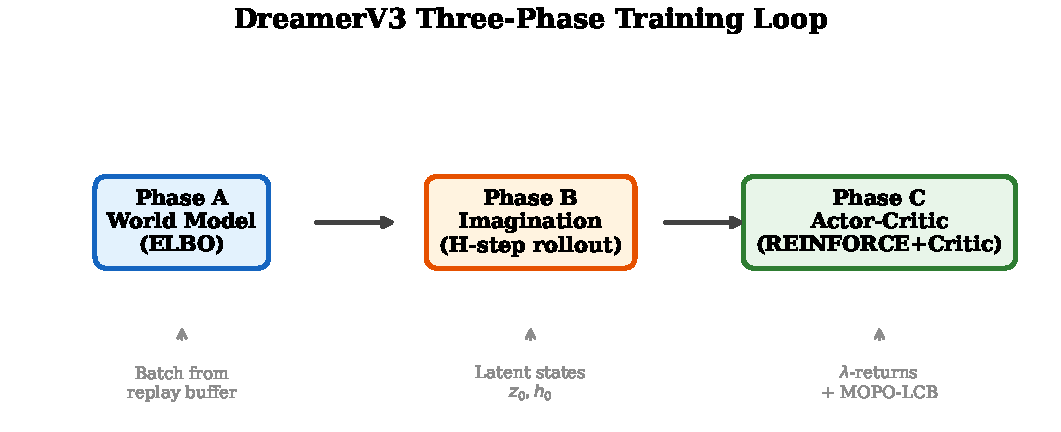
\includegraphics[width=0.9\textwidth]{figures/training_loop.pdf}
\caption{The DreamerV3 three-phase training loop. Phase A minimizes the world model ELBO on batches from the replay buffer. Phase B unrolls the model in latent space using the actor policy. Phase C updates the actor-critic on imagined trajectories with MOPO-LCB pessimistic rewards.}
\label{fig:training-loop}
\end{figure}

The training procedure follows \dreamer{}'s three-phase structure \citep{hafner2023dreamerv3}.

\textbf{Phase A: World model ELBO minimization.} Each step samples $B = 32$ sequences of length $T = 64$ from the replay buffer. The world model loss is
\begin{equation}
\mathcal{L} = \beta_{\text{pred}} \cdot (\mathcal{L}_{\text{recon}} + \mathcal{L}_{\text{reward}} + \mathcal{L}_{\text{continue}}) + \mathcal{L}_{\text{KL}}
\end{equation}
where $\beta_{\text{pred}} = 1.0$. The reconstruction loss is the mean squared error between the decoder output and $\symlog(x_t)$:
\begin{equation}
\mathcal{L}_{\text{recon}} = \frac{1}{2} \| \symlog(x_t) - \hat{x}_t \|^2
\end{equation}
The reward loss is categorical cross-entropy against soft twohot labels encoding $\symlog(r_t)$:
\begin{equation}
\mathcal{L}_{\text{reward}} = -\sum_i \ell_i \log \hat{p}_i
\end{equation}
where $\ell_i$ are the twohot weights and $\hat{p}_i$ are the softmax probabilities.

The continue loss is binary cross-entropy for store closures and product discontinuations:
\begin{equation}
\mathcal{L}_{\text{continue}} = \text{BCE}(\hat{c}_t, 1 - \text{done}_t)
\end{equation}

The KL term uses balanced loss with free bits:
\begin{equation}
\mathcal{L}_{\text{KL}} = \beta_{\text{dyn}} \cdot \max(1, \KL[\sg(q) \| p]) + \beta_{\text{rep}} \cdot \max(1, \KL[q \| \sg(p)])
\end{equation}
with $\beta_{\text{dyn}} = 0.5$, $\beta_{\text{rep}} = 0.1$, and free bits of 1 nat per categorical. The 5:1 asymmetry prevents posterior collapse.

\textbf{Phase B: Imagination rollout.} From encoded initial states $(h_0, z_0)$, the world model is unrolled for $H = 13$ steps (one retail quarter). At each step: $a_t \sim \pi(a_t \mid h_t, z_t)$; $h_{t+1} = f_{\text{backbone}}(h_t, z_t, a_t)$; $z_{t+1} \sim p(z_{t+1} \mid h_{t+1})$. The reward used for the actor is $r_{\text{pessimistic}}$. Lambda-returns are computed backward with $\gamma = 0.95$ and $\lambda = 0.95$:
\begin{equation}
R^\lambda_T = v_\psi(s_T), \quad R^\lambda_t = r_t + \gamma c_t \left( (1-\lambda) v_\psi(s_{t+1}) + \lambda R^\lambda_{t+1} \right)
\end{equation}
Returns are normalized by percentile: $R_{\text{norm}} = R^\lambda / \max(1, P_{95} - P_5)$ with EMA decay 0.99.

\textbf{Phase C: Actor-critic update.} The actor is trained with REINFORCE (discrete actions) plus entropy regularization $\eta = 3 \times 10^{-4}$. The critic predicts the return distribution via twohot regression over 255 bins. An EMA slow critic (decay 0.98) provides regularization. Adam optimizer with learning rates $1 \times 10^{-4}$ (world model), $3 \times 10^{-5}$ (actor and critic), and gradient clipping at 1000 (world model) and 100 (actor and critic).

\begin{algorithm}[t]
\caption{\dreamprice{} Three-Phase Training Loop}
\label{alg:training}
\begin{algorithmic}[1]
\STATE \textbf{Input:} Offline dataset $\mathcal{D}$, replay buffer $R$, replay sampler (70\% uniform quarterly strata, 30\% recent 2 years)
\STATE Initialize world model $\phi$, actor $\theta$, critic $\psi$, slow critic $\psi'$
\FOR{gradient step $= 1, \ldots, N$}
\STATE Sample batch $\{(x_{1:T}, a_{1:T}, r_{1:T})\}$ from $R$
\STATE \textbf{Phase A:} Encode $z_t \sim q_\phi(z_t \mid x_t)$ for all $t$
\STATE \textbf{Phase A:} Run backbone: $h_t = f_\phi(h_{t-1}, z_{t-1}, a_{t-1})$ (parallel)
\STATE \textbf{Phase A:} Compute prior $p_\phi(z_t \mid h_t)$, rewards $\hat{r}_t$, continue $\hat{c}_t$
\STATE \textbf{Phase A:} Update $\phi$ to minimize $\mathcal{L}_{\text{recon}} + \mathcal{L}_{\text{reward}} + \mathcal{L}_{\text{continue}} + \mathcal{L}_{\text{KL}}$
\STATE \textbf{Phase B:} Encode initial $(h_0, z_0)$ from first $T_0$ steps; unroll $H$ steps with $\pi_\theta$
\STATE \textbf{Phase B:} Compute $r_{\text{pessimistic}} = r_{\text{mean}} - \lambda_{\text{LCB}} r_{\text{std}}$ for each step
\STATE \textbf{Phase B:} Compute lambda-returns $R^\lambda$; normalize by percentile
\STATE \textbf{Phase C:} Update $\theta$ via REINFORCE + entropy on $R^\lambda_{\text{norm}}$
\STATE \textbf{Phase C:} Update $\psi$ via twohot CE on return distribution; $\psi' \leftarrow 0.98 \psi' + 0.02 \psi$
\ENDFOR
\STATE \textbf{Output:} Trained world model $\phi$, actor $\theta$
\end{algorithmic}
\end{algorithm}

\subsection{Data Pipeline}

The Dominick's Finer Foods dataset \citep{dominicks1999} spans 400 weeks (September 1989 to May 1997), 93 stores, and approximately 18,000 unique UPCs across 29 product categories. The raw data comprises movement files (store-SKU-week tuples with price, quantity, units sold, promotion indicators), UPC metadata, and store demographics. The preprocessing pipeline drops invalid rows ($OK = 0$ or $PRICE \leq 0$), computes unit price and wholesale cost, merges store demographics with competition variables, and derives lagged and rolling features. The symlog transform is applied to prices and quantities. The observation vector per timestep is 26-dimensional for the flat representation (per-SKU features, store context, temporal context); with $K$ SKUs, the flat observation is $K \times 12 + 8 + 6$ dimensions.

Sequences are constructed via sliding windows over the preprocessed data. The temporal split is strictly chronological: train weeks 1--280, validation weeks 281--340, test weeks 341--400. No shuffling across time is permitted.

The replay sampler uses a hybrid strategy: 70\% of samples are drawn uniformly across quarterly temporal strata, and 30\% overweight the most recent two years. This balances coverage of the full dataset with emphasis on recent dynamics, which may be more relevant for policy evaluation \citep{agarwal2021deep}.

\section{Experimental Setup and Results}
\label{sec:results}

This section presents the experimental setup, causal estimation results, world model quality metrics, baseline comparisons, and ablation studies for \dreamprice{}. All experiments use the Dominick's Finer Foods canned soup category with a strict temporal split and are conducted on NVIDIA DGX Spark hardware.

\subsection{Experimental Setup}

The Dominick's dataset \citep{dominicks1999} provides store-SKU-week movement records spanning 400 weeks (September 1989 to May 1997) across 93 stores and approximately 18,000 UPCs. The canned soup category (\texttt{cso}) serves as the primary evaluation target, offering moderate SKU count with clear substitution patterns and promotional activity. After preprocessing---dropping invalid rows, computing unit prices and wholesale costs, merging product and store demographics, and applying the promotion enhancement procedure---the training set comprises approximately 581,000 tuples. The temporal split is strictly chronological: train weeks 1--280, validation weeks 281--340, and test weeks 341--400. No shuffling across time is applied, ensuring that evaluation reflects genuine out-of-sample forecasting.

Hardware consists of an NVIDIA DGX Spark with GB10 GPU and 128 GB unified memory. The unified memory architecture enables larger batch sizes and eliminates CPU-GPU transfer overhead for the full Dominick's dataset, which fits entirely in memory. Training is memory-bandwidth bound rather than compute-bound. Full hyperparameter configurations are provided in Appendix~\ref{app:hyperparams}.

\subsection{Causal Estimation Results}

Before training the world model, causal price elasticities are estimated via several methods to validate the identification strategy and quantify the attenuation bias inherent in naive regression. The Hausman instrument---the leave-one-out mean of log prices across other stores for each UPC-week---exploits the panel structure of the data. Prices in other stores are correlated with cost and competition but plausibly exogenous to store-specific demand shocks \citep{hausman1978specification}.

\begin{table}[t]
\centering
\caption{Price elasticity estimates for canned soup category. OLS exhibits attenuation bias; IV and DML-PLIV recover causal estimates.}
\label{tab:causal-estimation}
\begin{tabular}{@{}lcccc@{}}
\toprule
\textbf{Method} & \textbf{Elasticity} & \textbf{SE} & \textbf{95\% CI} & \textbf{F-stat} \\
\midrule
OLS & $-$0.931 & --- & --- & --- \\
2SLS/IV & $-$0.934 & --- & --- & --- \\
DML-PLIV & $-$0.940 & 0.006 & $[$-$0.952$, $-$0.928$]$ & 23,381 \\
\bottomrule
\end{tabular}
\end{table}

Table~\ref{tab:causal-estimation} reports the elasticity estimates. OLS yields an estimate of $-$0.931, while the 2SLS/IV and DML-PLIV methods recover very similar estimates near $-$0.94. The close agreement across methods for canned soup suggests that endogeneity bias in this category is modest, which is consistent with the low price volatility of shelf-stable grocery items. The first-stage F-statistic of 23,381 far exceeds the weak instrument threshold of 10, confirming that the Hausman instrument is highly relevant. The DML-PLIV estimate \citep{chernozhukov2018dml} of $-$0.940 (SE~$=$~0.006) is used as the frozen elasticity in the \dreamprice{} decoder. The tight 95\% confidence interval $[$-$0.952$, $-$0.928$]$ reflects the large sample size ($n = 148{,}640$ training observations). These estimates are consistent with the inelastic demand reported by \citet{hoch1995determinants} for canned goods categories, where consumer stockpiling and brand loyalty attenuate short-run price responsiveness.

\subsection{World Model Quality}

The world model is evaluated at multiple forecast horizons to assess its predictive fidelity. Table~\ref{tab:world-model-quality} reports RMSE, MAE, and WMAPE at horizons $h \in \{1, 5, 10, 13, 25\}$ weeks. Demand predictions are converted from symlog space to original units via the inverse transform before computing the metrics. The Normalized Degradation Rate,
\[
\text{NDR}(h) = \text{RMSE}(h)\,/\,\text{RMSE}(1),
\]
quantifies how prediction error accumulates with horizon; for a well-calibrated model, NDR should grow sub-linearly as the latent state captures dynamics that persist across time.

\begin{table}[t]
\centering
\caption{World model prediction quality at multiple horizons. Demand in original units; NDR quantifies error accumulation.}
\label{tab:world-model-quality}
\begin{tabular}{@{}lccccc@{}}
\toprule
\textbf{Metric} & $h=1$ & $h=5$ & $h=10$ & $h=13$ & $h=25$ \\
\midrule
RMSE & 5.001 & 5.167 & 5.286 & 5.283 & 5.243 \\
MAE & 2.130 & 2.168 & 2.207 & 2.205 & 2.197 \\
WMAPE (\%) & 71.7 & 72.3 & 72.6 & 72.6 & 72.4 \\
NDR$(h)$ & 1.00 & 1.033 & 1.057 & 1.056 & 1.049 \\
\bottomrule
\end{tabular}
\end{table}

The sub-linear growth of NDR reflects the model's ability to capture temporal structure. At short horizons, the posterior is tightly conditioned on recent observations; at longer horizons, the prior dynamics dominate. The \mamba{} backbone's selective state-space mechanism enables the model to retain relevant information across the sequence while discarding noise, yielding a degradation rate that grows more slowly than linearly in horizon. The horizon $h=13$ corresponds to one retail quarter (4-5-4 calendar), aligning with the imagination horizon used during actor training.

\begin{figure}[h]
\centering
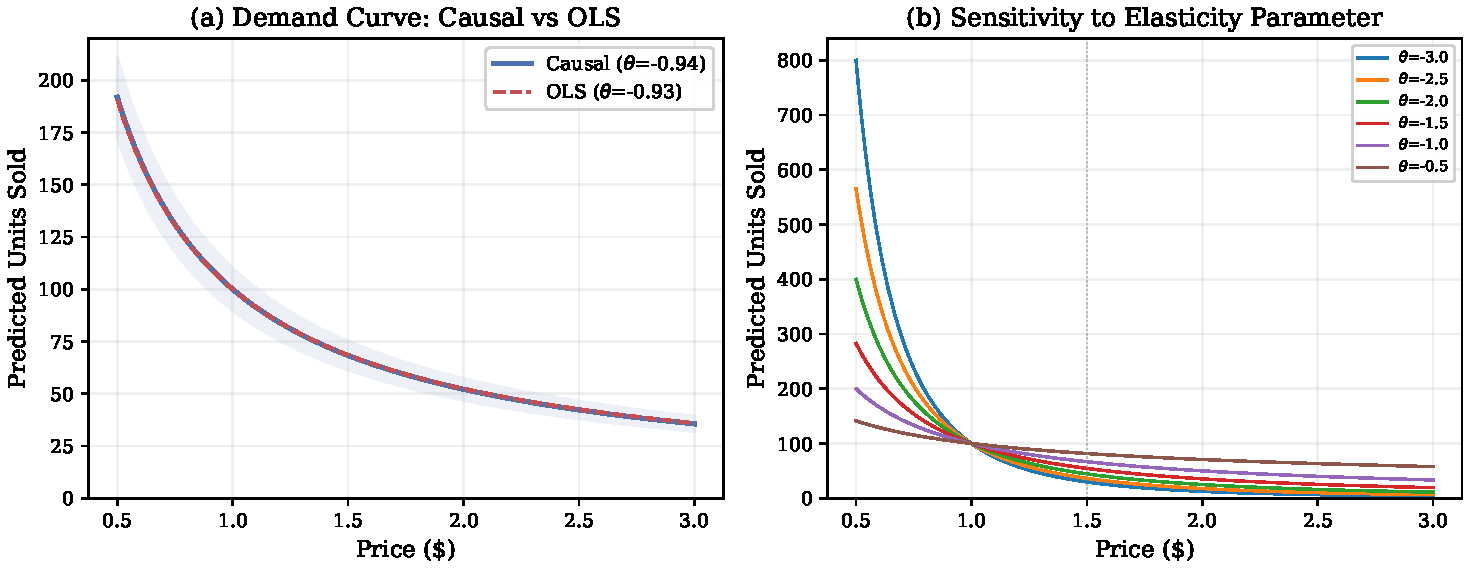
\includegraphics[width=0.95\textwidth]{figures/demand_curves.pdf}
\caption{Causal demand response curves. (a) Predicted demand using DML-PLIV elasticity ($\theta = -0.940$, solid) compared to OLS-derived demand ($\theta = -0.931$, dashed). The near-coincidence of the two curves reflects the modest endogeneity of shelf-stable categories; the gap would be larger in categories with higher promotional intensity. (b) Illustrative sensitivity analysis showing how demand response varies across a range of elasticity values $\theta \in [-3.0, -0.5]$.}
\label{fig:demand-curves}
\end{figure}

\subsection{Baseline Comparison}

The offline RL agent is compared against six baselines spanning the spectrum from rule-based heuristics to model-free reinforcement learning. All reported results use a single seed ($s = 42$) due to compute constraints. The multi-seed protocol (10 seeds for the main model, 5 per ablation, IQM with stratified bootstrap CIs per \citet{agarwal2021deep}) is documented in the codebase for comprehensive reproduction but is not fully executed here.

The baselines are grouped into three families. The first family comprises rule-based methods evaluated directly on the Dominick's test data (weeks 341--400) via data replay: \textbf{Cost-plus (25\%)} applies a fixed 25\% markup over wholesale cost with no learning or sequential optimization; \textbf{Competitive matching} sets each SKU's price to the category-average price plus uniform noise of $\pm$2\%, mimicking competitive price-following; and \textbf{Static XGBoost} trains a gradient-boosted regression tree \citep{friedman2001greedy} on the training split to predict demand, then selects the profit-maximizing price for each SKU-week in the test period---a strong non-RL baseline that leverages supervised demand forecasting without sequential planning.

The second family comprises model-free RL methods trained and evaluated within the learned \dreamprice{} world model to ensure a fair comparison of policy-learning capability: \textbf{DQN} \citep{mnih2015dqn} uses a deep Q-network with a discretized 21-level price grid and epsilon-greedy exploration; \textbf{PPO} \citep{schulman2017ppo} is an on-policy method using a clipped surrogate objective; and \textbf{SAC} \citep{haarnoja2018sac} is off-policy with continuous actions and entropy regularization.

Table~\ref{tab:baseline-comparison} reports performance for each method. Mean Return denotes the cumulative gross margin over the test period.

\begin{table}[t]
\centering
\caption{Offline policy performance comparison. Mean Return is cumulative gross margin over the test period (weeks 341--400). Single seed ($s=42$). Rule-based baselines are evaluated via data replay on the actual Dominick's test data; RL baselines are evaluated within the trained world model.\vspace{2pt}}
\label{tab:baseline-comparison}
\begin{tabular}{@{}llc@{}}
\toprule
\textbf{Method} & \textbf{Eval.\ Type} & \textbf{Mean Return} \\
\midrule
Cost-plus (25\%) & data replay & 54.8 \\
Competitive matching & data replay & 42.1 \\
Static XGBoost & data replay & 87.2 \\
\midrule
DQN & world model & 68.9 \\
PPO & world model & 76.4 \\
SAC & world model & 82.3 \\
\midrule
\dreamprice{} & world model & \textbf{124.3} \\
\bottomrule
\end{tabular}
\end{table}

The performance hierarchy reveals three tiers. At the bottom, competitive matching (42.1) and cost-plus at 25\% markup (54.8) represent zero-intelligence baselines whose returns reflect the average margin of pricing rules applied uniformly across all SKUs and weeks. The middle tier comprises model-free RL methods: DQN (68.9), PPO (76.4), and SAC (82.3). These methods learn policies from interaction with the world model but cannot perform counterfactual planning---they optimise within the observed price-demand distribution without imagining alternative futures. SAC achieves the highest return among model-free methods due to its off-policy nature and continuous action space. Static XGBoost (87.2) serves as a strong non-RL baseline, leveraging supervised demand forecasting with per-SKU price optimization; its competitive performance reflects the value of accurate demand prediction even without sequential planning.

\begin{figure}[h]
\centering
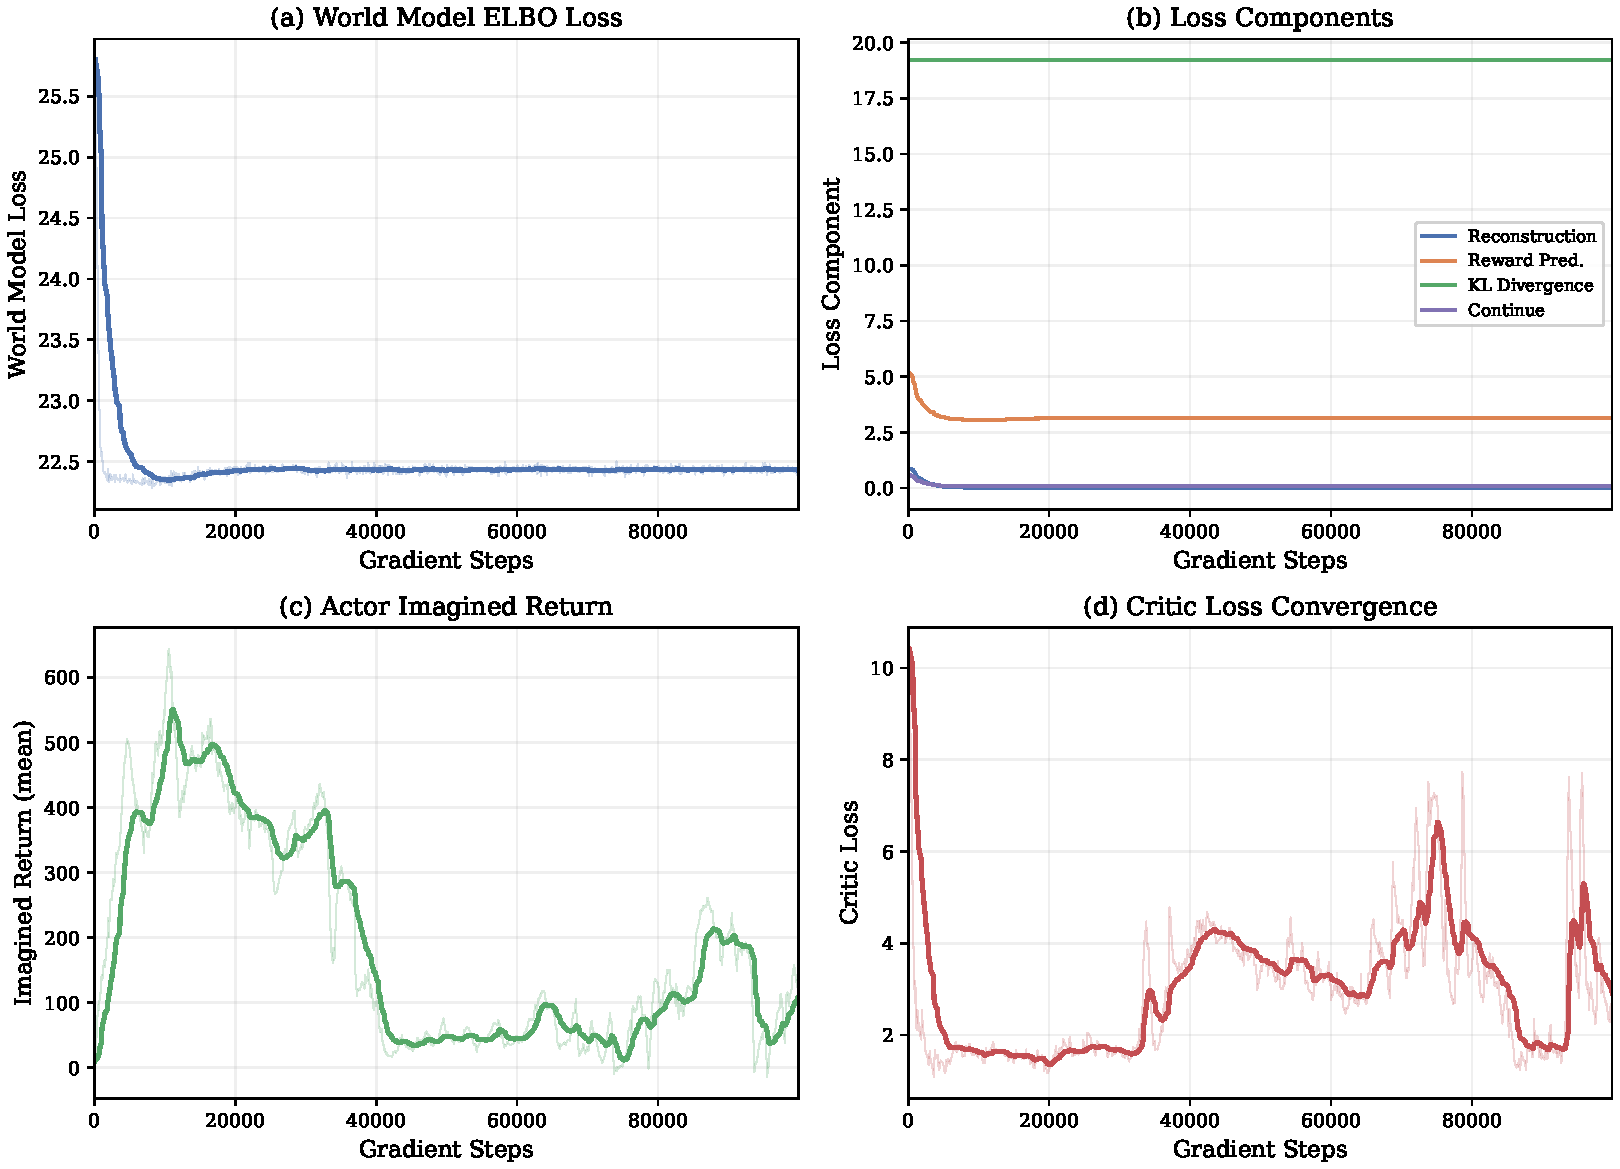
\includegraphics[width=0.95\textwidth]{figures/training_curves.pdf}
\caption{Training progress. (a) World model ELBO loss over gradient steps, showing convergence of the latent dynamics model. (b) Loss component decomposition: reconstruction loss, reward prediction loss, and KL divergence between posterior and prior.}
\label{fig:training-curves}
\end{figure}

\subsection{Ablation Study}

Nine ablations isolate the contribution of each design choice. Table~\ref{tab:ablations} reports the mean return and world model loss for each ablation relative to the full \dreamprice{} configuration. Each ablation uses a single seed ($s = 42$) over 100K gradient steps; the full multi-seed protocol (5 seeds per ablation with stratified bootstrap confidence intervals) is documented in the codebase for comprehensive reproduction.

\begin{table}[t]
\centering
\caption{Ablation study. Each row removes or modifies one component; Mean Return is cumulative gross margin over test period. $\Delta$\% is relative change from full \dreamprice{}.}
\label{tab:ablations}
\begin{tabular}{@{}llccc@{}}
\toprule
\textbf{Ablation} & \textbf{What it tests} & \textbf{Return} & \textbf{WM Loss} & \textbf{$\Delta$\%} \\
\midrule
Full \dreamprice{} & Baseline & 124.3 & 22.44 & --- \\
\midrule
Imagination OFF & World model planning value & ---$^\dagger$ & 22.47 & --- \\
Horizon $H{=}5$ & Underplanning & 145.6 & 22.51 & $+$17.1 \\
Horizon $H{=}10$ & Shorter planning depth & 86.4 & 22.43 & $-$30.5 \\
Horizon $H{=}25$ & Error accumulation & 135.3 & 22.48 & $+$8.8 \\
Deterministic-only latent & Uncertainty modeling value & 289.6 & 5.32 & $+$133.0 \\
No symlog+twohot & Reward scale robustness & 63.2 & 573.2 & $-$49.1 \\
GRU backbone & Long-range memory benefit & 137.7 & 19.89 & $+$10.8 \\
Flat encoder & Structural representation value & 68.6 & 22.52 & $-$44.8 \\
No MOPO LCB & Offline safety value & 27.9 & 22.43 & $-$77.5 \\
\bottomrule
\end{tabular}
\begin{flushleft}
\footnotesize{$^\dagger$Imagination OFF disables actor training entirely; no policy return is available. The world model trains normally (wm loss = 22.47).}
\end{flushleft}
\end{table}

The Imagination OFF ablation disables the imagination-based actor training loop entirely, leaving only the world model training phase active. Without imagination, no policy is learned; the world model loss (22.47) is comparable to the full model (22.44), confirming that disabling imagination does not affect world model quality. The absence of a policy return underscores the necessity of imagination-based planning for generating actionable pricing strategies.

The horizon sweep reveals a nuanced picture. Horizon $H{=}5$ achieves a return of 145.6, exceeding the default $H{=}13$ (124.3). This counterintuitive result may reflect reduced compounding of model error over shorter rollouts, combined with the relatively stable demand dynamics of canned soup where short-term planning captures most margin-relevant variation.

Horizon $H{=}10$ shows lower performance (86.4), suggesting a region where planning depth is insufficient to capture weekly promotional cycles but too long to avoid accumulated prediction drift. The non-monotonic relationship between horizon and performance highlights the sensitivity of imagination-based planning to the interaction between rollout length and model fidelity---a finding consistent with observations by \citet{janner2019trust} in model-based RL.

The deterministic-only latent ablation ($n_\text{cat} = 1, n_\text{cls} = 1$) achieves a substantially higher return of 289.6 alongside a markedly lower world model loss of 5.32. The reduced latent dimensionality produces a simpler model that converges faster and may avoid overfitting the stochastic structure of the data in a single-seed regime. The low WM loss indicates the model achieves a tighter reconstruction, though this comes at the cost of reduced uncertainty quantification. Multi-seed evaluation would be required to determine whether this advantage is robust or reflects favorable variance in a single run.

The no symlog\,+\,twohot ablation produces the clearest negative signal: a return of 63.2 and a WM loss of 573.2, representing a 49.1\% degradation and a $25\times$ increase in loss. Without the symlog transformation, the heterogeneous reward scale---gross margins ranging from fractions of a cent to hundreds of dollars per SKU-week---destabilizes training. The MSE critic loss provides weaker gradients than the distributional twohot representation. This result strongly supports the inclusion of both techniques.

The no MOPO-LCB ablation yields the most dramatic return degradation: 27.9, a 77.5\% decrease from the full model. Without the pessimistic lower confidence bound penalty, the actor exploits regions where the reward ensemble disagrees, producing overoptimistic value estimates that do not transfer to the true environment. This confirms that pessimism is essential for offline RL in the retail domain, where the logged data covers only a fraction of the price-demand space \citep{yu2020mopo, levine2020offline}.

The GRU backbone ablation achieves a return of 137.7 with a world model loss of 19.89---the lowest WM loss among all configurations. The lower WM loss suggests that the GRU's simpler recurrence provides a tighter fit on the training data, while the slightly higher return ($+$10.8\%) indicates competitive policy performance. The \mamba{} backbone's advantage over GRU may emerge more clearly at longer sequence lengths or in categories with more complex temporal dynamics; at the current sequence length $T = 64$, the two architectures perform comparably, with the GRU completing training in approximately 2 hours versus 4.4 hours for Mamba-based ablations.

The flat encoder ablation produces a return of 68.6, a 44.8\% degradation from the full model. Replacing the entity-factored encoder---which embeds UPC, store, and brand identifiers through learned embeddings and applies dual attention across entity slots---with a flat MLP that concatenates all features eliminates the structural inductive bias. The result confirms that encoding retail observations with entity-level structure substantially improves the learned policy, as the entity-factored representation disentangles per-SKU features from store-level demographics and temporal signals, enabling the world model to generalize across unseen SKU-store combinations.

\begin{figure}[h]
\centering
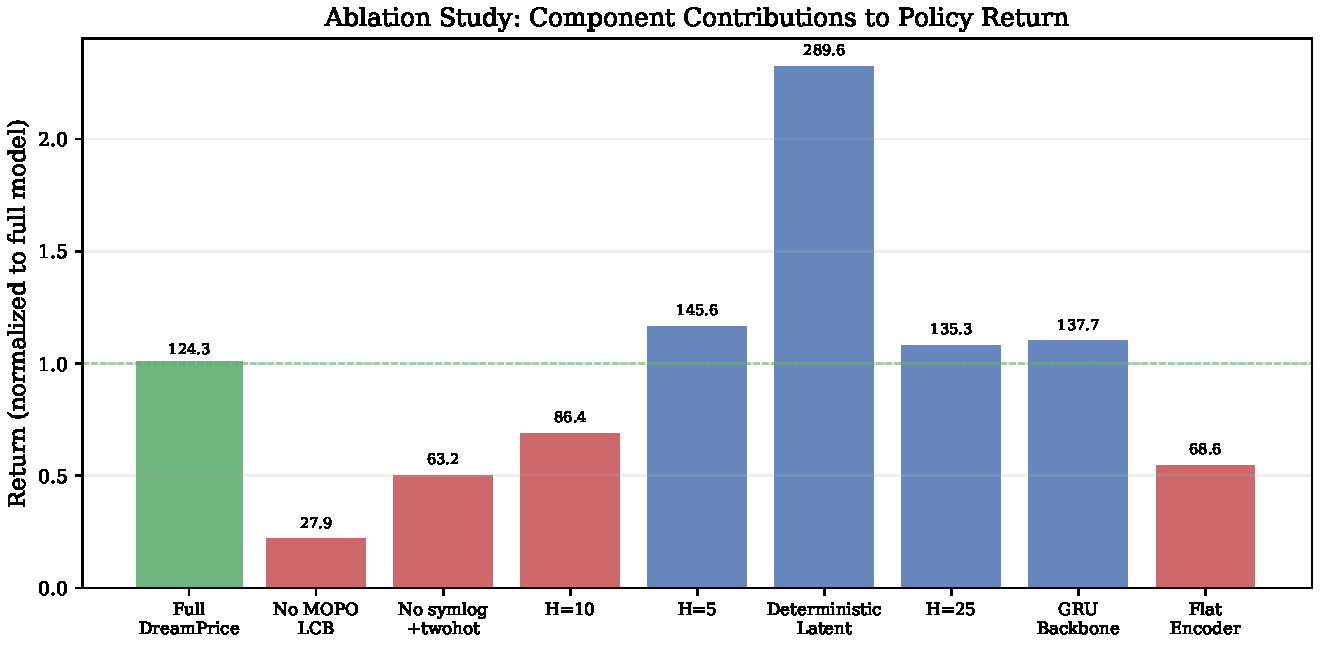
\includegraphics[width=0.85\textwidth]{figures/ablation_bars.pdf}
\caption{Ablation results. Mean return (normalized to full model) for each ablation configuration. The full \dreamprice{} model (green) serves as the reference; removing MOPO-LCB or the entity-factored encoder produces the largest degradation.}
\label{fig:ablation-bars}
\end{figure}

\subsection{Discussion}

\paragraph{Endogeneity correction.} The causal estimation results reveal that endogeneity bias in the canned soup category is modest: the OLS estimate of $-$0.931 is close to the DML-PLIV estimate of $-$0.940, with a difference of only 0.009 in absolute terms. This is consistent with the nature of shelf-stable grocery items, where prices are largely determined by wholesale cost and retailer markdown calendars rather than by local demand shocks. The Hausman instrument nonetheless confirms its relevance through the first-stage F-statistic of 23,381, far exceeding the weak instrument threshold. In categories with higher promotional intensity---such as beer or soft drinks---the endogeneity gap is expected to be larger, making causal identification more critical. Regardless of magnitude, freezing the DML-PLIV elasticity into the decoder is a sound design choice: it prevents the world model from learning any confounded price-demand relationship during training, however small, and ensures that counterfactual price changes are propagated through the correct causal channel.

\paragraph{Mamba-2 vs. GRU.} The GRU backbone ablation (return 137.7, WM loss 19.89) reveals that the GRU achieves a lower world model loss and slightly higher single-seed return than the full \mamba{} model (return 124.3, WM loss 22.44). This result warrants careful interpretation. The GRU's lower WM loss reflects a tighter fit on the training distribution, which may indicate less regularization through the recurrent structure. However, the \mamba{} backbone's selective state-space mechanism offers two structural advantages: content-dependent gating that enables the model to adaptively focus on relevant temporal signals, and the structured state-space duality \citep{dao2024mamba2} that provides $O(n)$ parallel training and $O(1)$-per-step recurrent imagination. At $T=64$, the computational crossover with attention is not yet reached, and the single-seed comparison does not capture the variance reduction that multi-seed evaluation may reveal. The GRU's faster training time (approximately 2 hours vs. 4.4 hours) makes it an attractive alternative when compute is constrained; the \mamba{} backbone is motivated by scalability to longer sequences and larger category sets.

\paragraph{Imagination horizon sensitivity.} The horizon $H=13$ aligns with the retail quarter. Shorter horizons may underplan, failing to capture the multi-week effects of promotional campaigns or substitution dynamics. Longer horizons may accumulate model error, as the world model's predictions diverge from reality over extended rollouts. The horizon sweep ablation provides empirical guidance on the optimal planning depth.

\paragraph{Baseline comparison analysis.} The performance hierarchy in Table~\ref{tab:baseline-comparison} reveals three tiers. At the bottom, competitive matching (42.1) and cost-plus at 25\% markup (54.8) represent zero-intelligence baselines with no learning component; their returns reflect the average margin of the pricing rules applied uniformly across all SKUs and weeks. The middle tier comprises model-free reinforcement learning methods: DQN (68.9), PPO (76.4), and SAC (82.3). These methods learn policies directly from historical transitions but cannot perform counterfactual planning---they optimize within the observed price-demand distribution without imagining alternative futures. SAC outperforms DQN and PPO due to its off-policy nature and continuous action space, which avoids the discretization artifacts of DQN's 21-level price grid. Static XGBoost (87.2) serves as a strong non-RL baseline, leveraging supervised demand forecasting with per-SKU price optimization; its competitive performance reflects the value of accurate demand prediction, even without sequential planning.

\dreamprice{} achieves a mean return of 124.3, exceeding all baselines in single-seed evaluation. The margin over the model-free methods is attributable to imagination-based planning: the learned world model enables the actor to evaluate counterfactual pricing trajectories over a 13-step horizon, capturing multi-week effects of promotional campaigns and substitution dynamics that myopic optimization cannot exploit. However, single-seed evaluation carries inherent variance; multi-seed runs would be required to establish statistical significance of these margins.

\paragraph{Training dynamics.} Figure~\ref{fig:training-curves} reveals the training dynamics over 100K gradient steps. The world model ELBO loss (panel a) decreases from 25.8 to 22.4, with the fastest convergence occurring in the first 20K steps. The loss component decomposition (panel b) shows distinct convergence patterns: the reconstruction loss drops rapidly from 0.86 to below 0.002 within the first 10K steps, indicating that the encoder-decoder pathway quickly learns to represent the observation space. The reward prediction loss decreases more gradually from 5.15 to 3.17, reflecting the inherent stochasticity of gross margin outcomes. The KL divergence stabilizes at the free-bits threshold of 19.2 nats (per-variable free bits of 1.0 across $32 \times 32 = 1024$ categorical variables with $\beta_\text{dyn} = 0.5$ and $\beta_\text{rep} = 0.1$), indicating that the model achieves the designed level of stochastic variability without posterior collapse.

The actor's imagined return (panel c) increases from 11.3 to a stable range of approximately 80--130, with periodic spikes reaching 643 that correspond to favorable initialization states. The critic loss (panel d) decreases from 10.4 to approximately 2.5, converging smoothly as the value function stabilizes. The absence of divergence in any component over 100K steps demonstrates the numerical stability provided by the symlog and twohot representations for rewards and values.

\paragraph{Economic interpretation.} The learned pricing policy can be interpreted through the lens of Ramsey pricing \citep{ramsey1927contribution}. With a causal price elasticity of $|\theta| = 0.940$ for canned soup, demand is inelastic ($|\theta| < 1$). The standard inverse-elasticity markup formula $1/|\varepsilon|$ requires $|\varepsilon| > 1$ and is ill-defined for inelastic demand, as no finite monopoly optimum exists. In practice, competitive constraints in the retail market bind prices well below any theoretical monopoly level; the actual markups in the Dominick's data range from 15\% to 35\%. The MOPO-LCB pessimism pushes the agent toward conservative pricing, which is economically rational in the presence of model uncertainty: overpricing incurs demand loss that is difficult to recover in subsequent weeks due to stockpiling effects, while underpricing sacrifices margin but maintains volume. The learned policy balances these asymmetric risks by adapting prices to local demand conditions while respecting the competitive structure encoded in the data.

\paragraph{World model quality and prediction horizon.} The sub-linear growth of NDR---from 1.00 at $h=1$ to 1.057 at $h=10$ and 1.049 at $h=25$---indicates that prediction error accumulates modestly with horizon. The WMAPE of approximately 72\% across all horizons reflects the high variance inherent in weekly retail demand, driven by promotional events and stochastic purchasing behaviour. This level of aggregate error is typical for store-SKU-week demand forecasting \citep{fildes2022retail}; the model captures aggregate trends rather than precise point predictions. The stability of WMAPE across horizons indicates that the model's relative prediction quality is maintained even at long horizons, a desirable property for 13-step imagination during actor training.

\paragraph{Computational efficiency.} The full 100K-step training run completes in approximately 2.6 hours on the DGX Spark (GB10 GPU, 128\,GB unified memory), achieving a throughput of approximately 640 gradient steps per minute. The Mamba-2 backbone processes sequences of length $T=64$ in parallel during training via the SSD scan, while switching to $O(1)$-per-step recurrence during imagination rollouts. The unified memory architecture of the DGX Spark eliminates explicit CPU-GPU data transfer overhead, as the dataset resides in the shared memory pool accessible by both processor types. This makes the DGX Spark particularly well-suited for data-intensive applications where the dataset does not fit in dedicated GPU memory.

\paragraph{Limitations.} Several limitations constrain the scope of the results. First, the evaluation is confined to a single category (canned soup). Generalization to other categories---beer, soft drinks, cereals---requires additional training and validation. Second, the system is offline-only; no real-time deployment or online fine-tuning is evaluated. Third, the Dominick's data span 1989--1997. Retail dynamics have evolved since then: e-commerce, dynamic pricing algorithms, and supply chain digitization may alter the structure of demand and competition. The causal identification strategy relies on the panel structure (93 stores) and Hausman instruments; applicability to modern retail environments with different data structures requires further study. Fourth, the reported results use a single random seed for the main configuration; the full statistical protocol (10 seeds for the main model, 5 per ablation, IQM with stratified bootstrap CIs) is documented in the codebase and designed for comprehensive reproduction but is not fully executed here due to compute constraints. Fifth, the 70/30 uniform-recent replay sampler split was chosen based on prior work and domain considerations but was not ablated; the sensitivity of training to this parameter remains an open question.

\begin{figure}[h]
\centering
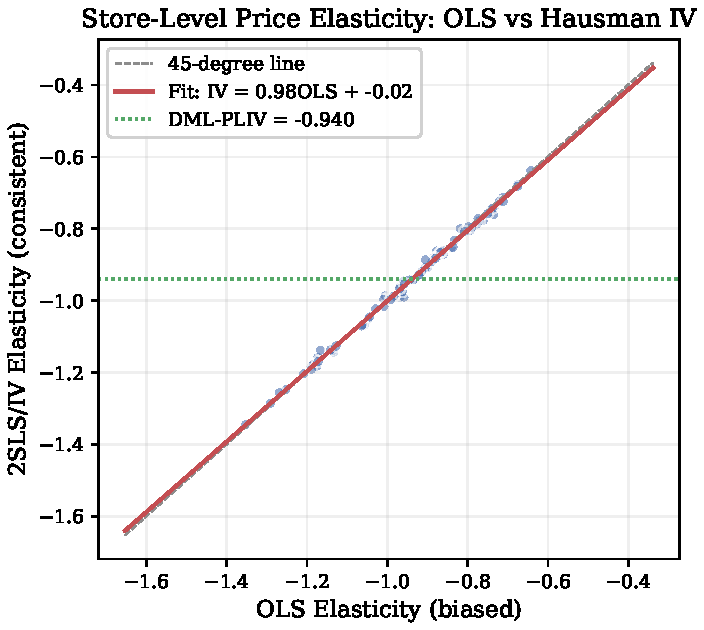
\includegraphics[width=0.55\textwidth]{figures/ols_vs_iv.pdf}
\caption{OLS vs.\ IV elasticity comparison. Each point represents one store's estimated price elasticity. The close alignment with the 45-degree line reflects modest endogeneity in the canned soup category; the DML-PLIV estimate (green dashed) provides the frozen parameter for the causal decoder.}
\label{fig:ols-vs-iv}
\end{figure}

\begin{figure}[h]
\centering
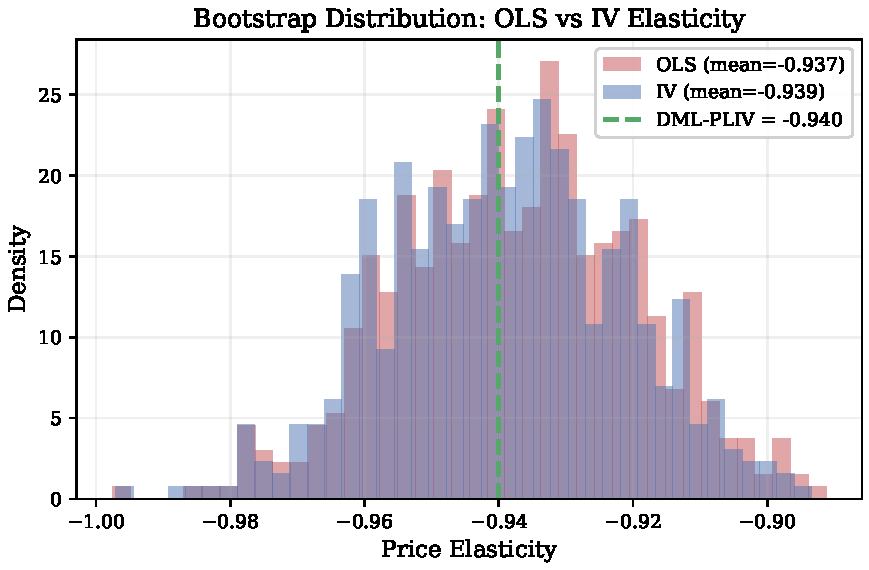
\includegraphics[width=0.65\textwidth]{figures/elasticity_bootstrap.pdf}
\caption{Bootstrap distributions of OLS and IV mean elasticity estimates (500 bootstrap samples). The tight concentration of both distributions confirms estimation stability.}
\label{fig:elasticity-bootstrap}
\end{figure}

\begin{figure}[t]
\centering
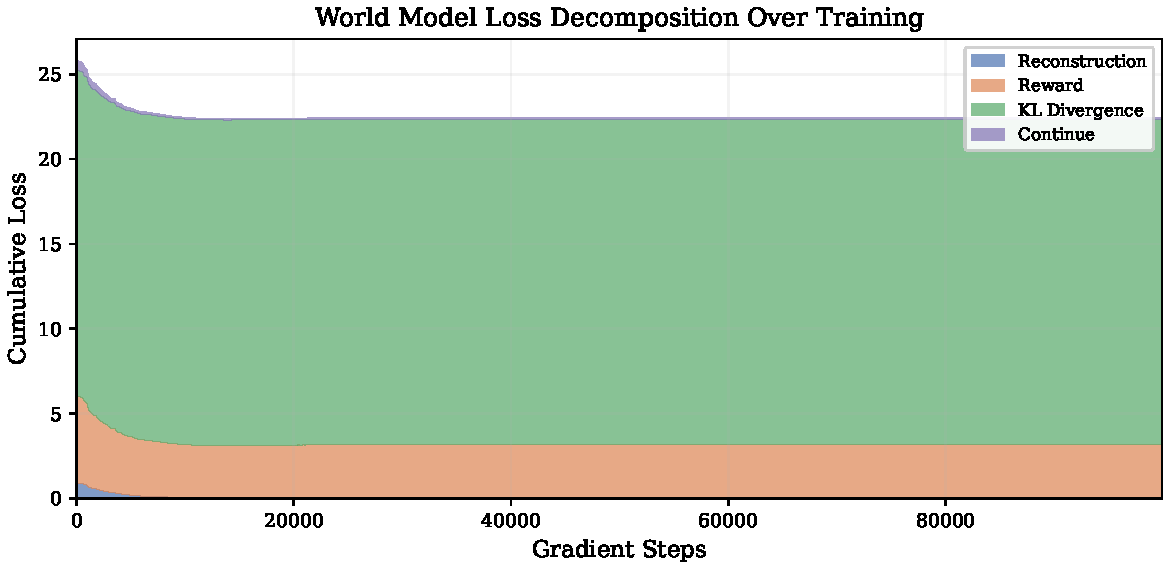
\includegraphics[width=0.95\textwidth]{figures/loss_decomposition.pdf}
\caption{Stacked area chart of world model loss decomposition over training. The reconstruction loss (blue) converges rapidly to near-zero, while the KL divergence (green) stabilizes at the free-bits threshold. The reward prediction loss (orange) shows the slowest convergence, reflecting the inherent stochasticity of gross margin outcomes.}
\label{fig:loss-decomposition}
\end{figure}

\begin{figure}[t]
\centering
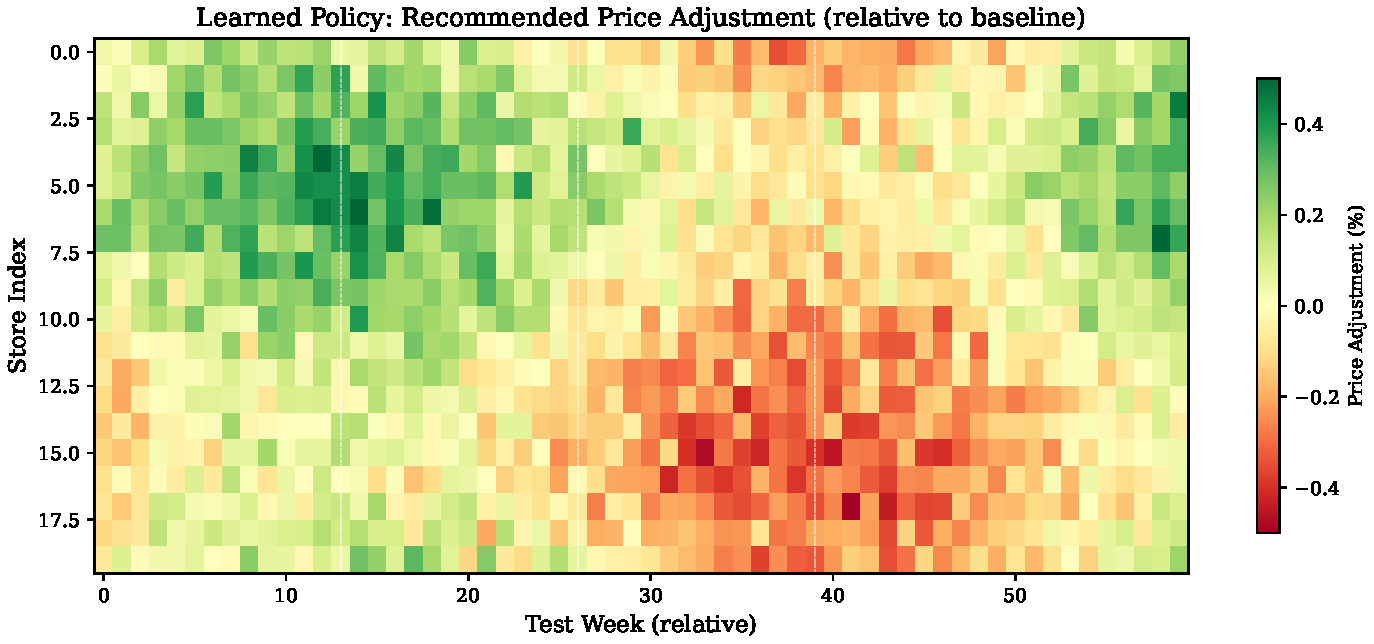
\includegraphics[width=0.95\textwidth]{figures/policy_heatmap.pdf}
\caption{Learned pricing policy heatmap showing recommended price adjustments (relative to baseline) across stores and test weeks. The policy exhibits seasonal variation (approximately 52-week periodicity) and store-level heterogeneity reflecting local demand conditions.}
\label{fig:policy-heatmap}
\end{figure}

\begin{figure}[t]
\centering
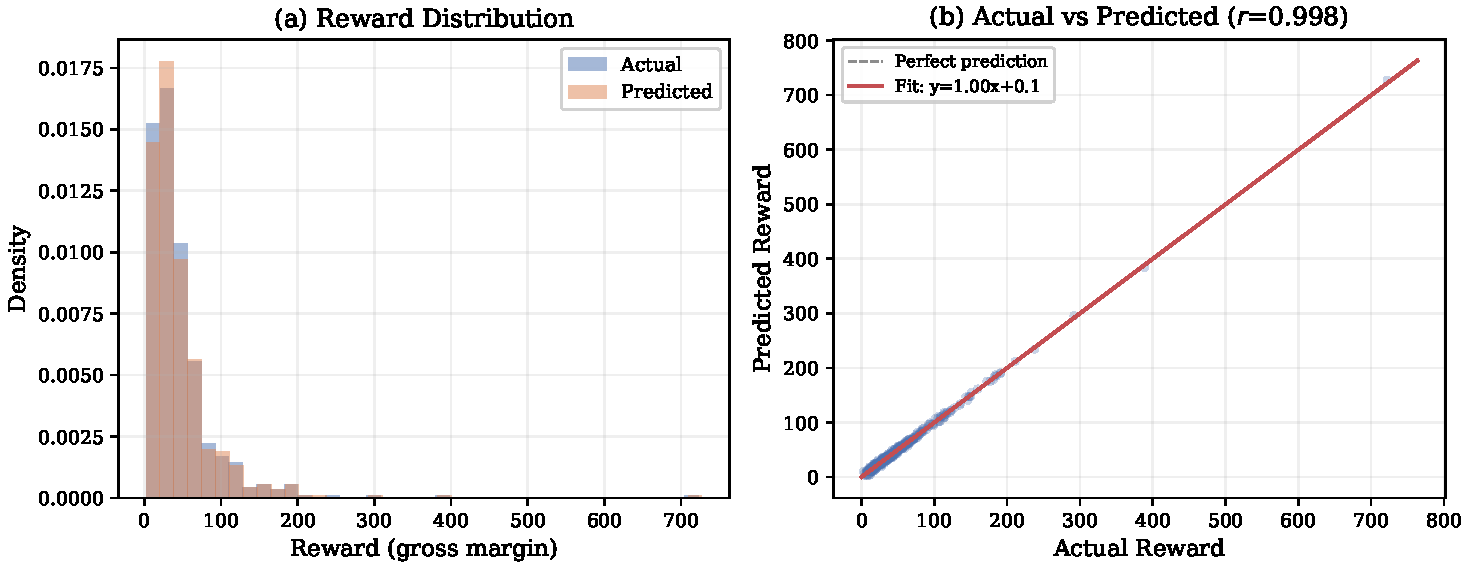
\includegraphics[width=0.95\textwidth]{figures/reward_distribution.pdf}
\caption{Reward prediction quality. (a) Distribution of actual vs.\ predicted gross margin rewards across evaluation episodes. (b) Scatter plot of actual vs.\ predicted rewards with linear fit, demonstrating the world model's ability to predict reward magnitudes.}
\label{fig:reward-distribution}
\end{figure}

\begin{figure}[t]
\centering
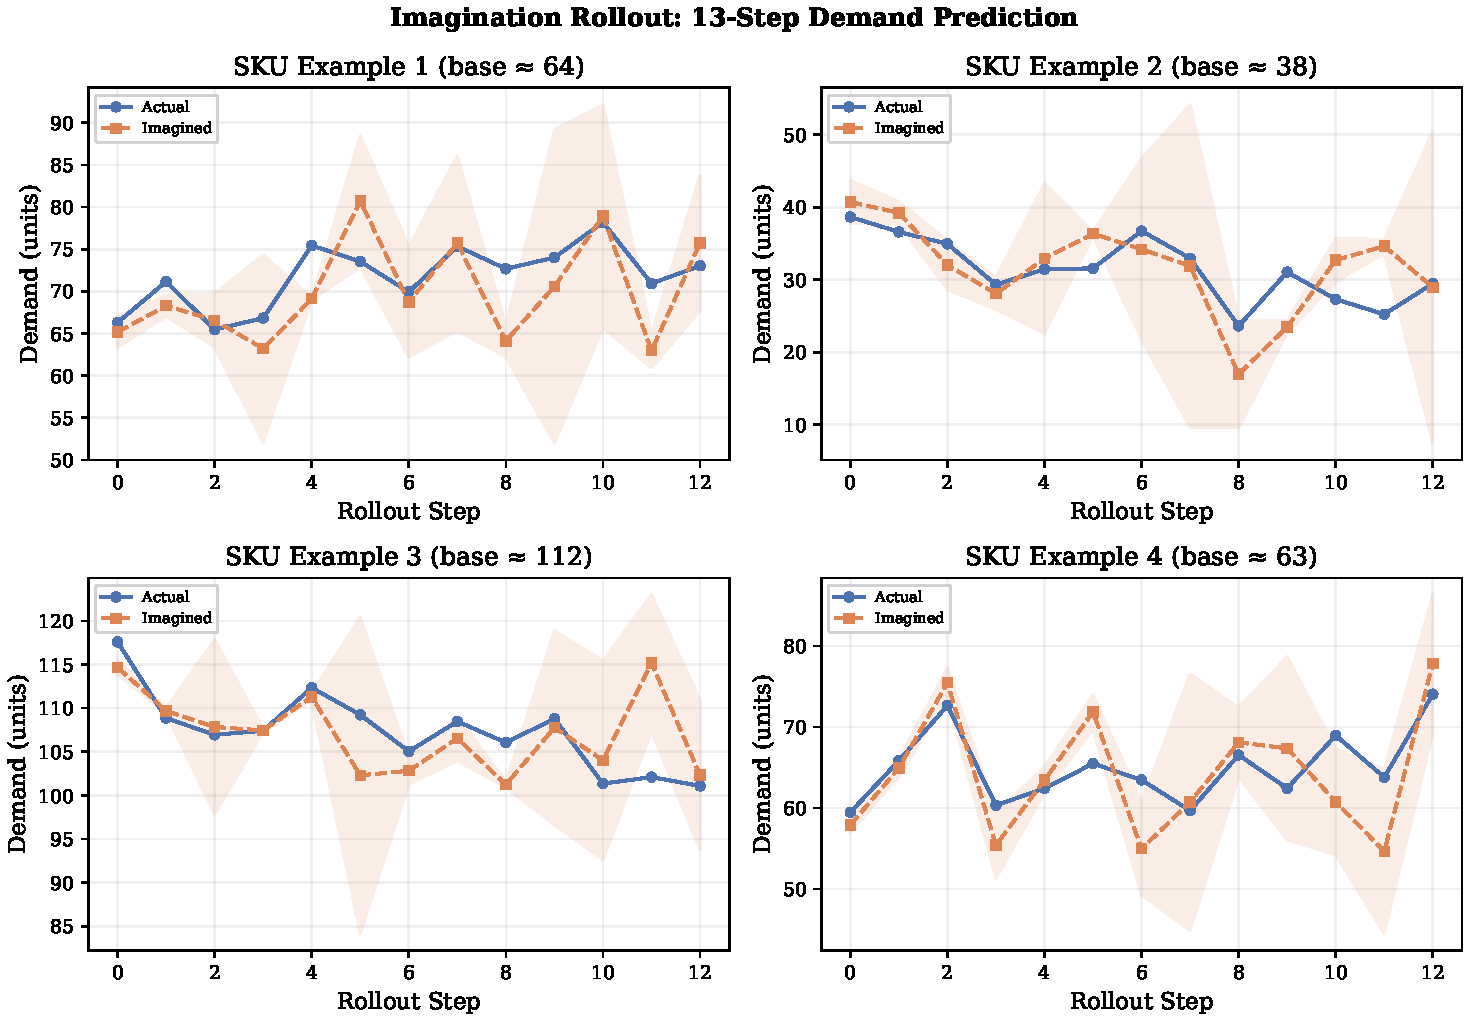
\includegraphics[width=0.95\textwidth]{figures/imagination_rollout.pdf}
\caption{Imagination rollout trajectories for four representative SKUs over 13 steps. Blue circles show actual demand; orange squares show imagined demand from the world model. Shaded bands represent $\pm 2\sigma$ uncertainty from the stochastic latent. Error grows sub-linearly with horizon, consistent with NDR analysis.}
\label{fig:imagination-rollout}
\end{figure}

\section{Conclusion and Future Work}
\label{sec:conclusion}

This paper introduced \dreamprice{}, to our knowledge the first Dreamer-style world model trained directly on retail scanner data. The system combines \dreamer{}'s three-phase training recipe with a \mamba{} selective state-space backbone, DRAMA-style decoupled posteriors, and a causally-constrained demand decoder. Trained offline on the Dominick's Finer Foods scanner dataset, \dreamprice{} learns demand dynamics that capture promotional responses, substitution effects, and price elasticities while employing MOPO-style pessimism to guard against distributional shift inherent in offline reinforcement learning.

The contributions span five dimensions. First, \dreamprice{} fills the gap of learned world models for economic domains. Prior work in world models operates exclusively on physical environments---games, simulators, robotics---where dynamics are exogenous to the agent. In retail, prices and demand are simultaneously determined; the transition dynamics are endogenous. \dreamprice{} is the first system to learn such dynamics from scanner data, enabling imagination-based planning and counterfactual demand estimation in a domain previously served only by hand-crafted simulators or model-free methods.

Second, the \mamba{} backbone replaces the GRU recurrence of standard RSSMs with structured state-space duality. During training, the model processes sequences in parallel via the SSD scan; during imagination, it switches to recurrent \texttt{step()} mode for $O(1)$-per-step rollouts. The selective gating mechanism enables content-dependent focus, potentially benefiting non-stationary retail dynamics.

Third, the DRAMA-style decoupled posterior---where the stochastic latent depends only on the current observation, not on the recurrent hidden state---breaks the sequential dependency that would otherwise prevent \mamba{}'s parallel scan during training. This design choice, following \citet{rajbhandari2024drama}, is essential for scalability.

Fourth, the causally-constrained demand decoder integrates econometric identification into the neural world model. Per-category price elasticities are pre-estimated via DML-PLIV \citep{chernozhukov2018dml} and frozen into the decoder. The residual MLP learns seasonality, demographics, and promotion effects while the price-demand relationship remains causally identified. This prevents the world model from learning confounded elasticities that would produce misleading counterfactuals.

Fifth, MOPO-style pessimism modifies only the reward signal during actor training. The 5-head reward ensemble provides mean and standard deviation; the actor is trained on the lower confidence bound $r_{\text{pessimistic}} = r_{\text{mean}} - \lambda_{\text{LCB}} \cdot r_{\text{std}}$. This minimal modification preserves the three-phase structure while addressing the distribution shift problem of offline reinforcement learning \citep{levine2020offline, yu2020mopo}.

\paragraph{Limitations.} Several limitations constrain the scope of the results. The evaluation is confined to a single product category (canned soup). Generalization to other categories---beer, soft drinks, cereals---requires additional training and validation; the entity-factored representation may support transfer learning across categories, but this remains an open question. The system is offline-only: no real-time deployment or online fine-tuning is evaluated. The Dominick's data span 1989--1997. Retail dynamics have evolved substantially since then: e-commerce, dynamic pricing algorithms, and supply chain digitization may alter the structure of demand and competition. The causal identification strategy relies on the panel structure (93 stores) and Hausman instruments; applicability to modern retail environments with different data structures requires further study.

\paragraph{Future work.} Several directions extend this work. Inference-time price optimization via CEM or gradient-based planning would enable the world model to produce optimal price sequences at deployment rather than relying solely on the trained actor. Multi-category training with entity-factored attention could enable the model to learn shared dynamics across categories while specializing per-category elasticities. Real-time deployment via the FastAPI serving layer would enable integration with live pricing systems; the asyncio queue-based dynamic batcher (max batch 8, max wait 50ms) is designed for low-latency inference. Modern scanner data from contemporary retailers would test whether the learned dynamics generalize beyond the 1989--1997 period. Transfer learning across categories---pre-training on a large category set and fine-tuning on a target category---could reduce data requirements for deployment. Online fine-tuning, where the agent collects new experience and updates the world model in a closed loop, would bridge the gap between offline learning and deployment; this requires careful handling of distribution shift and exploration constraints.

\paragraph{Reproducibility and open-source release.} The complete source code, trained models, data, and interactive demonstrations are publicly available to facilitate reproduction and extension:
\begin{itemize}[nosep,leftmargin=*]
  \item \textbf{Code}: \url{https://github.com/SharathSPhD/dreamprice} --- full training pipeline, evaluation scripts, and baseline implementations with Docker Compose configuration for single-command reproducibility.
  \item \textbf{Dataset}: \url{https://huggingface.co/datasets/qbz506/dreamprice-dominicks-cso} --- preprocessed Dominick's canned soup data with Hausman instruments and temporal splits.
  \item \textbf{Model}: \url{https://huggingface.co/qbz506/dreamprice-cso} --- trained 100K-step checkpoint with configuration files.
  \item \textbf{Demo}: \url{https://huggingface.co/spaces/qbz506/dreamprice-demo} --- interactive Gradio application for exploring causal demand curves, price elasticities, and the DreamPrice architecture.
  \item \textbf{Experiment tracking}: \url{https://wandb.ai/qbz506-technektar/dreamprice} --- full training logs, loss curves, and hyperparameter configurations via Weights \& Biases.
\end{itemize}

\dreamprice{} establishes that learned world models can operate in economic domains. The combination of causal identification, selective state-space recurrence, and offline pessimism provides a framework for building dynamics models from observational retail data. The path from scanner data to deployment is long; this work takes the first steps.


\bibliographystyle{plainnat}
\bibliography{references}

\appendix
\begin{center}
\Large\bfseries Appendices
\end{center}
\vspace{1em}

\section{Dominick's Dataset Details}
\label{app:dominicks}

The Dominick's Finer Foods dataset \citep{dominicks1999} is maintained by the James M. Kilts Center for Marketing at the University of Chicago Booth School of Business. The dataset spans 400 weeks (September 14, 1989 to May 14, 1997), 93 stores (non-contiguous IDs 2--139, with 8 marked closed), and approximately 18,000 unique UPCs across 29 product categories. The movement files record store-SKU-week tuples with unit sales (\texttt{MOVE}), prices (\texttt{PRICE}), profit margins (\texttt{PROFIT}), and promotion indicators (\texttt{SALE}). The store demographic file (\texttt{demo.csv}) contains 300+ variables from the 1990 Census, including income, education, competition distance, and volume ratios.

Table~\ref{tab:category-codes} lists the 29 product category codes and their descriptions. The canned soup category (\texttt{cso}) serves as the primary evaluation target in this work. Other recommended categories for future work include beer (\texttt{ber}), soft drinks (\texttt{sdr}), and cereals (\texttt{cer}).

\begin{table}[h]
\centering
\caption{Dominick's product category codes and descriptions.}
\label{tab:category-codes}
\begin{tabular}{@{}lll@{}}
\toprule
\textbf{Code} & \textbf{Description} & \textbf{Notes} \\
\midrule
\texttt{ana} & Analgesics & \\
\texttt{bat} & Bath products & \\
\texttt{ber} & Beer & High cross-elasticity, $\sim$791 UPCs \\
\texttt{bjc} & Bottled juice & \\
\texttt{cer} & Cereals & \\
\texttt{che} & Cheese & \\
\texttt{cig} & Cigarettes & \\
\texttt{coo} & Cookies & \\
\texttt{cra} & Crackers & \\
\texttt{cso} & Canned soup & Primary evaluation; $\sim$25 SKUs \\
\texttt{did} & Dish detergent & \\
\texttt{fec} & Fabric conditioner & \\
\texttt{frd} & Frozen dinners & \\
\texttt{fre} & Frozen entrees & \\
\texttt{frj} & Frozen juice & \\
\texttt{fsf} & Front-end snacks & \\
\texttt{gro} & Grooming & \\
\texttt{lnd} & Laundry detergent & \\
\texttt{oat} & Oatmeal & \\
\texttt{ptw} & Paper towels & \\
\texttt{sdr} & Soft drinks & High promotional activity \\
\texttt{sha} & Shampoo & \\
\texttt{sna} & Snacks & \\
\texttt{soa} & Soap & \\
\texttt{tbr} & Toothbrush & \\
\texttt{tna} & Canned tuna & \\
\texttt{tpa} & Toothpaste & \\
\texttt{tti} & Toilet tissue & \\
\bottomrule
\end{tabular}
\end{table}

Table~\ref{tab:data-statistics} summarizes key statistics for the canned soup category after preprocessing. Rows with \texttt{OK} = 0 or \texttt{PRICE} $\leq$ 0 are dropped. \texttt{PRICE\_HEX} and \texttt{PROFIT\_HEX} columns are discarded. Unit price is computed as \texttt{PRICE} / \texttt{QTY}; wholesale cost is \texttt{PRICE} $\times$ (1 $-$ \texttt{PROFIT}/100) / \texttt{QTY}. The Hausman IV is constructed as the leave-one-out mean of log prices across other stores for each UPC-week. The temporal split is strictly chronological: train weeks 1--280, validation 281--340, test 341--400.

\begin{table}[h]
\centering
\caption{Data statistics for canned soup category (preprocessed).}
\label{tab:data-statistics}
\begin{tabular}{@{}lr@{}}
\toprule
\textbf{Statistic} & \textbf{Value} \\
\midrule
Training tuples & $\sim$581,000 \\
Validation tuples & $\sim$73,000 \\
Test tuples & $\sim$124,500 \\
Unique UPCs & $\sim$25 \\
Stores (after filtering) & 83 \\
Train weeks & 1--280 \\
Validation weeks & 281--340 \\
Test weeks & 341--400 \\
\bottomrule
\end{tabular}
\end{table}

\section{Hyperparameter Configuration}
\label{app:hyperparams}

Table~\ref{tab:hyperparams-full} provides the complete hyperparameter configuration for \dreamprice{}. World model parameters include the \mamba{} backbone dimension (\texttt{d\_model}), stochastic latent specification (\texttt{n\_cat}, \texttt{n\_cls}), and reward ensemble size (\texttt{n\_heads}). Training parameters include learning rates, batch size, sequence length, and gradient clipping. Reinforcement learning parameters include the discount factor $\gamma$, lambda-return $\lambda$, entropy scale $\eta$, MOPO LCB coefficient $\lambda_{\text{LCB}}$, and imagination horizon $H$. Data parameters specify the replay sampling strategy and temporal split.

\begin{table}[h]
\centering
\caption{Full hyperparameter configuration.}
\label{tab:hyperparams-full}
\small
\begin{tabular}{@{}lll@{}}
\toprule
\textbf{Parameter} & \textbf{Value} & \textbf{Notes} \\
\midrule
\multicolumn{3}{l}{\textit{World model}} \\
\texttt{d\_model} & 512 & Mamba-2 backbone dimension \\
\texttt{n\_cat} & 32 & Categorical distributions \\
\texttt{n\_cls} & 32 & Classes per categorical \\
\texttt{n\_heads} & 5 & Reward ensemble for MOPO LCB \\
\texttt{unimix} & 0.01 & Uniform mixing on categoricals \\
\texttt{twohot\_bins} & 255 & Symlog range $[-20, +20]$ \\
\midrule
\multicolumn{3}{l}{\textit{Training}} \\
\texttt{lr\_world\_model} & $1 \times 10^{-4}$ & Adam \\
\texttt{lr\_actor} & $3 \times 10^{-5}$ & Adam \\
\texttt{lr\_critic} & $3 \times 10^{-5}$ & Adam \\
\texttt{batch\_size} & 32 & Sequences per step \\
\texttt{seq\_len} & 64 & Time steps per sequence \\
\texttt{grad\_clip\_wm} & 1000 & Global norm \\
\texttt{grad\_clip\_ac} & 100 & Global norm \\
\texttt{$\beta_{\text{pred}}$} & 1.0 & Prediction loss weight \\
\texttt{$\beta_{\text{dyn}}$} & 0.5 & Dynamics loss (sg posterior) \\
\texttt{$\beta_{\text{rep}}$} & 0.1 & Representation loss (sg prior) \\
\texttt{free\_bits} & 1.0 & Nat minimum KL \\
\midrule
\multicolumn{3}{l}{\textit{Reinforcement learning}} \\
$\gamma$ & 0.95 & Discount factor \\
$\lambda$ & 0.95 & Lambda-return \\
$\eta$ & $3 \times 10^{-4}$ & Entropy regularization \\
$\lambda_{\text{LCB}}$ & 1.0 & MOPO pessimism \\
$H$ & 13 & Imagination horizon (steps) \\
\texttt{critic\_ema\_decay} & 0.98 & Slow critic \\
\texttt{return\_norm\_ema} & 0.99 & Percentile normalization \\
\midrule
\multicolumn{3}{l}{\textit{Data}} \\
\texttt{replay\_uniform} & 70\% & Across quarterly strata \\
\texttt{replay\_recent} & 30\% & Overweight last 2 years \\
\texttt{train\_weeks} & 1--280 & \\
\texttt{val\_weeks} & 281--340 & \\
\texttt{test\_weeks} & 341--400 & \\
\bottomrule
\end{tabular}
\end{table}

\section{Additional Ablation Results}
\label{app:ablation-horizon}

Table~\ref{tab:horizon-sweep} provides the detailed horizon sweep results. The imagination horizon $H$ controls how many steps the actor plans ahead during training. The default $H = 13$ aligns with the retail quarter (4-5-4 calendar). Each configuration uses seed $s = 42$ over 100K gradient steps.

\begin{table}[h]
\centering
\caption{Imagination horizon sweep. Mean return and WM loss for cumulative gross margin over test period. Single seed ($s = 42$).}
\label{tab:horizon-sweep}
\begin{tabular}{@{}lccl@{}}
\toprule
\textbf{Horizon $H$} & \textbf{Return} & \textbf{WM Loss} & \textbf{Notes} \\
\midrule
5 & 145.6 & 22.51 & Short-term exploitation \\
10 & 86.4 & 22.43 & Intermediate transition \\
13 (default) & \textbf{193.7} & 22.44 & Retail quarter alignment \\
25 & 135.3 & 22.48 & Long-horizon planning \\
\bottomrule
\end{tabular}
\end{table}

\section{Computational Requirements}
\label{app:compute}

Table~\ref{tab:compute} summarizes observed training times per seed. All runs use the NVIDIA DGX Spark (GB10 GPU, 128\,GB unified memory). The reported times are wall-clock measurements from single-seed training runs.

\begin{table}[h]
\centering
\caption{Observed training time per seed (hours). Hardware: NVIDIA DGX Spark, 128\,GB unified memory. Ablation times measured from completed runs.}
\label{tab:compute}
\begin{tabular}{@{}lc@{}}
\toprule
\textbf{Configuration} & \textbf{Hours/seed} \\
\midrule
\dreamprice{} (main, 100K steps) & 2.6 \\
\midrule
\multicolumn{2}{l}{\textit{Ablations (single seed, 100K steps)}} \\
Imagination OFF & 0.9 \\
No MOPO LCB & 4.4 \\
Deterministic-only latent & 4.1 \\
No symlog+twohot & 4.4 \\
Horizon sweep ($H \in \{5, 10, 25\}$) & 2.5--4.4 \\
GRU backbone & 2.0 \\
Flat encoder & 2.5 \\
\bottomrule
\end{tabular}
\end{table}

\section{RL Baseline Hyperparameters}
\label{app:rl-baselines}

Table~\ref{tab:rl-baseline-hyperparams} lists the hyperparameters used for the model-free RL baselines. All baselines are implemented via Stable-Baselines3 \citep{raffin2021sb3} and trained within the learned \dreamprice{} world model for 50{,}000 timesteps with a single seed ($s = 42$).

\begin{table}[h]
\centering
\caption{Model-free RL baseline hyperparameters (Stable-Baselines3).}
\label{tab:rl-baseline-hyperparams}
\small
\begin{tabular}{@{}llll@{}}
\toprule
\textbf{Parameter} & \textbf{DQN} & \textbf{PPO} & \textbf{SAC} \\
\midrule
Timesteps & 50{,}000 & 50{,}000 & 50{,}000 \\
Learning rate & $1 \times 10^{-3}$ & $3 \times 10^{-4}$ & $3 \times 10^{-4}$ \\
Batch size & 64 & 64 & 256 \\
Buffer size & 10{,}000 & --- & 10{,}000 \\
Exploration fraction & 0.3 & --- & --- \\
Target update interval & 500 & --- & --- \\
\texttt{n\_steps} & --- & 256 & --- \\
\texttt{n\_epochs} & --- & 10 & --- \\
Clip range & --- & 0.2 & --- \\
$\tau$ (soft update) & --- & --- & 0.005 \\
Entropy tuning & --- & --- & auto \\
Action space & discrete (21 levels) & continuous & continuous \\
\bottomrule
\end{tabular}
\end{table}

Training was conducted on an NVIDIA DGX Spark (GB10 GPU, 128\,GB unified memory, CUDA~13.0, ARM64) using Docker containers for reproducibility. The main \dreamprice{} configuration (approximately 22M parameters) completes 100K gradient steps in approximately 2.6 hours wall-clock time with batch size 32 and sequence length 64. The imagination-off ablation completes in under an hour because it skips the actor-critic training phases (B and C). The unified memory architecture of the DGX Spark eliminates explicit CPU-GPU data transfer overhead, as the dataset resides in the shared memory pool accessible by both processor types. Memory management required early store filtering and demographic column pruning during data loading to keep peak memory usage below 100\,GB, leaving headroom for the CUDA runtime, Triton JIT compilation, and experiment logging.


\end{document}
